\newpage \section{Introduction}
\label{sec:intro}





Given these challenges, research in machine learning on source code~\cite{allamanis2018:survey} tends to focus on restricted domain-specific languages~\cite{chen2021:latent,flashmeta,liventsev2021:bf} or automating specific parts\footnote{~similarly to autonomous driving~\cite{grigorescu2020:survey,marcano2020:review}} of the software development process~\cite{lu2021:codexglue,niu2023:crosscodebench} such as code search~\cite{husain2020:codesearchnet}, code translation~\cite{roziere2020:unsupervised}, detection of issues~\cite{fernandes2016:reviewbased,chakraborty2021:deep}, improvement~\cite{petke2018:genetic} and repair~\cite{gouesAutomatedProgramRepair2019} rather than fully autonomous programming in a programming language popular with human developers~\cite{:tiobe}.
However, two recent innovations potentially make the latter task tractable.

\begin{figure*}
    \centering
    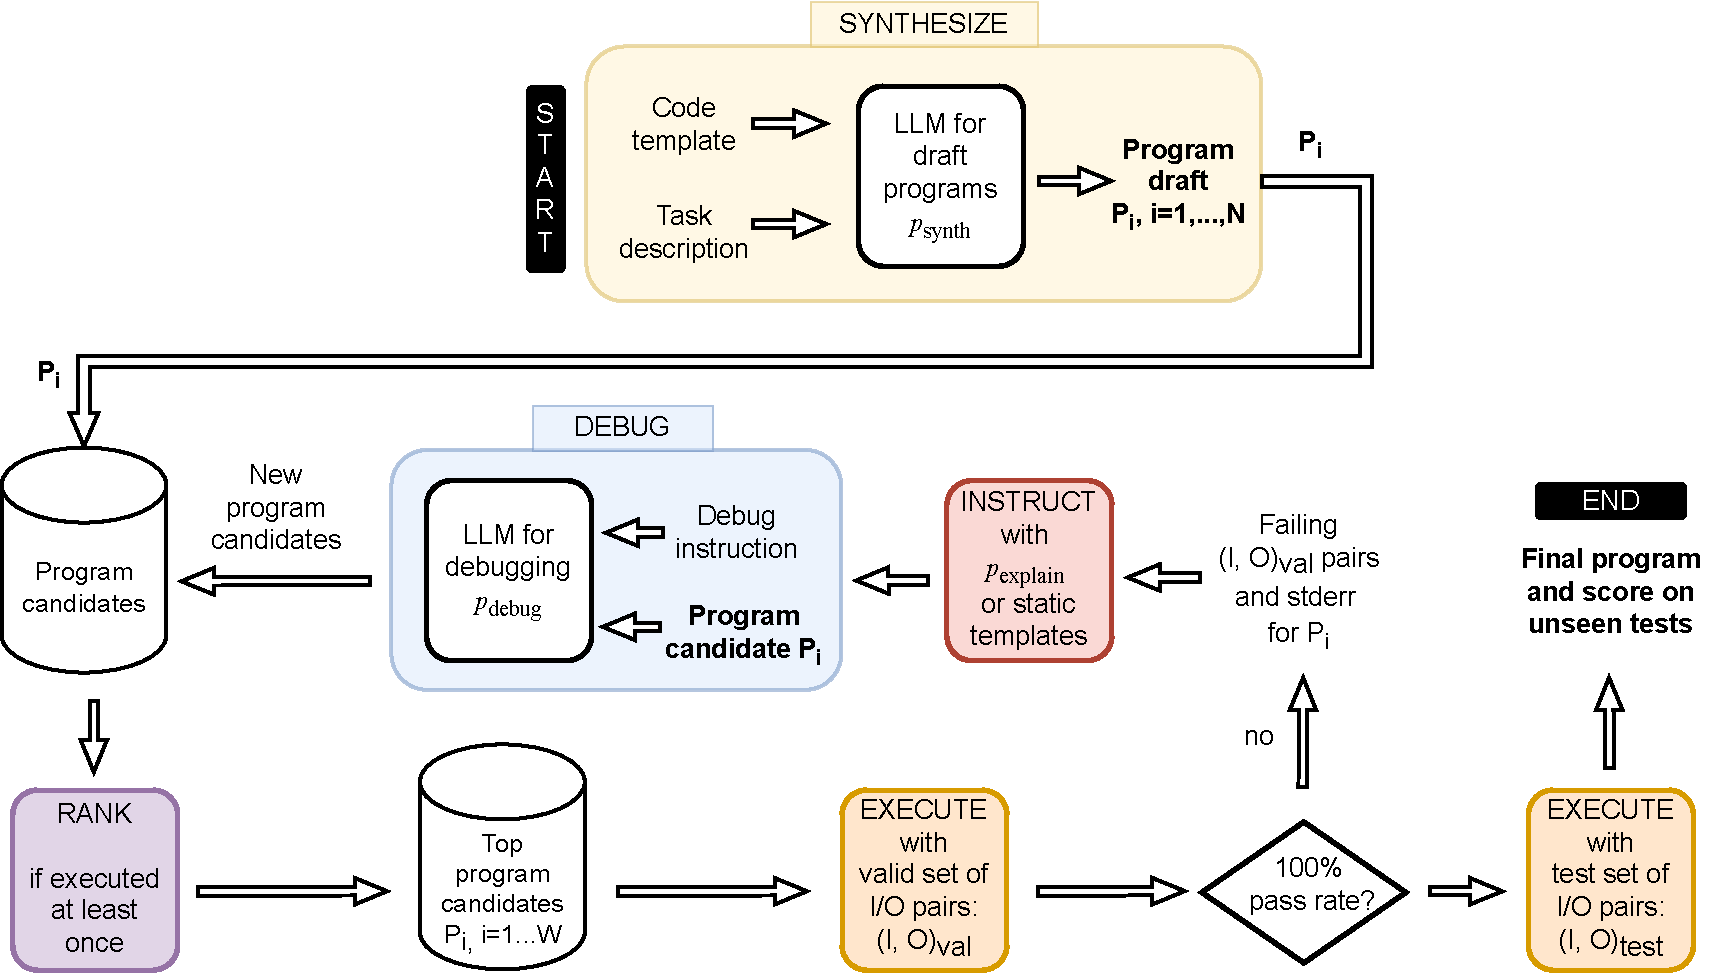
\includegraphics[width=\linewidth,trim={0mm 8mm 0mm 0mm}]{codex-for-psb-seidr-methodology-4.drawio.pdf}
    \caption{Overview of Synthesize, Execute, Instruct, Debug, and Rank}
    \label{fig:method}
\end{figure*}

One is \emph{Synthesize, Execute, Debug}~\cite{guptaSynthesizeExecuteDebug2020}, a framework that attempts to bridge the "last mile" gap by introducing program repair into the program synthesis algorithm. 
A programming task is specified using both a natural language description and a set of input/output (I/O) pairs demonstrating what output is expected of the program, thereby combining text to code ~\cite{iyer2018:mapping} and programming by example~\cite{halbertProgrammingExample1984,gulwani2016:programming} paradigms typical for competitive programming~\cite{zavershynskyi2018:naps}.
\emph{Synthesize, Execute, Debug} creates a first draft program using a generative model, compiles and executes it with given input examples.
This is followed by a program repair step to fix the identified errors.

Another relevant innovation is instruction fine-tuned large language models~\cite{ouyang2022:training}. Instruction fine-tuned models use human feedback in their training process and are designed to explicitly or implicitly admit two inputs: a source text (or code) and a textual command instructing the model to edit the source in a particular way, i.e., "summarize" or "translate to Python".
These models have been shown to be highly successful in automatic program repair~\cite{fanAutomatedRepairPrograms2023}. 
However, given the free-form nature of these instructions\footnote{Throughout this chapter we avoid other definitions of \emph{instruction}, such as \emph{an individual operation in code}, to prevent ambiguity.} how one should engineer instructions that maximize repair performance is an open question. 

Section~\ref{sec:seidr-methodology} presents a framework that adapts \emph{Synthesize, Execute, Debug} to instruction fine-tuned Large Language Models in agents for solving programming tasks in an autonomous fashion. 
We discuss related work in Section~\ref{sec:related-work}, introduce experiments to establish optimal search and prompting strategies for this framework in Section~\ref{sec:eval}. 
Finally, we demonstrate in Section~\ref{sec:results} that our framework outperforms conventional automatic programming techniques, such as genetic programming and naive application of large language models that generate one solution per problem without updating it iteratively. 

\newpage \section{Methodology}
\label{sec:seidr-methodology}
The proposed 5-agent framework, \emph{Synthesize, Execute, Instruct, Debug and Rank}, or \method{},\footnote{~seiðr also refers to a type of Norse magic~\cite{blain2002:nine} pertaining to predicting and controlling the future, which we deem thematically appropriate.} is summarized in figure \ref{fig:method}, which we discuss in detail in Section~\ref{sec:ingredients}.
To solve a programming task defined as a text description and a collection of I/O examples, we split I/O examples into prompt and validation sets and use the prompt set in a large language model to \synthesize{} a population of candidate solutions.
We \execute{} the solutions, test them against the validation set, generate a text description of the identified problems used to \instruct{} a large language model to produce repaired candidate solutions similar to the way a human developer \debug{}s a program.
We \rank{} the candidates
by correctness measured by matching I/O pairs, discard the worst candidates, and repeat until a fully correct solution is found.

 

\newpage \subsection{Ingredients}
\label{sec:ingredients}

\method{} makes use of instruction fine-tuned large language models: a \emph{synthesis} model \synthmodel{}, a \emph{debugging} model \debugmodel{}, as well as a model \textmodel{} that can be used for writing textual instructions, which are forwarded to the code generation model \debugmodel{} for code updates. 
Therefore, the setup can be described as two agents communicating with each other, whereby one generates code and another one provides critical or supervising comments on what should be changed in the generated code. 

The models \synthmodel{}, \debugmodel{}, and \textmodel{} can be either separate models or the same model.
The pre-requisites are that \synthmodel{} and \debugmodel{} models are able to understand natural language (descr) and partial or full programs (code) and generate code based on them. 
The model \textmodel{} should be able to understand code and natural language and either auto-complete or generate the debugging instruction from scratch. 
Note that the debugging instructions can be generated from failing tests using static templates 
%as described in~\cite{liventsev2023:fully}. 
However, we focus on the implementation in which an LLM generates debug instructions, which is also suitable for chat models in addition to instruction fine-tuned models. 
In general, \method{} requires a sequence-to-sequence generative model for these agents. 
We have chosen the state-of-the-art transformer models~\cite{vaswani2017:attention} for \synthmodel{}, \debugmodel{}, and \textmodel{} in our experiments as described in Section~\ref{sec:models}. 

Each LLM is a highly parameterised probability distribution over the space of (code, description)-tuples with parameters estimated on a large diverse (i.e., non-task-specific) corpus.
This stochastic nature of language models is an important prerequisite for \method{}, since it lets us sample batches of diverse candidate solutions from \synthmodel{}, \debugmodel{}, and \textmodel{}. 
We denote the number of generated outputs with $\treearitydraft{},$ $\treearitydebug{},$ and $\treearityexplain{},$ correspondingly.
Moreover, each model generates the most probable and less probable outputs in each batch, which helps diversify problem solving attempts. 
In the implementation-related sections further, we explain how we vary with the number of candidate solutions, debug instructions, and repairs generated in a batch by each LLM in \method{}.


\paragraph{Synthesize}
\label{sec:synth}

\begin{figure}
    \centering
    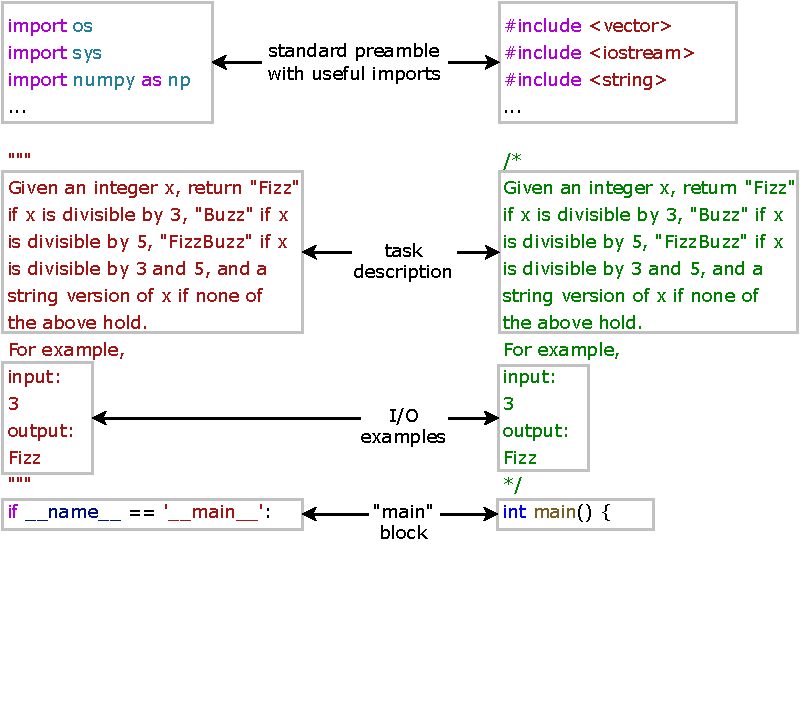
\includegraphics[width=0.7\linewidth, trim={0mm 40mm 0mm 0mm}, clip]{Templates-new-v2.pdf}
    \caption{Anatomy of \synthesize{} templates}
    \label{fig:template}
\end{figure}

The framework starts with the \synthesize{} agent, which is responsible for generating initial draft solutions to programming tasks to be repaired in the later stages of \method{}.
We start with a basic template for a chosen programming language that contains a number of standard library imports as shown in figure~\ref{fig:template}.
We populate this template with a comment indicating a text description of a task at hand and several I/O examples from the prompt training set.
We design the templates with prompt engineering guidelines\footnote{\url{https://platform.openai.com/docs/guides/prompt-engineering/six-strategies-for-getting-better-results}}$^{,}$ and prior work (chapter \ref{ch:tree2tree} in mind.
We then sample $\treearitydraft{}$ programs from \synthmodel{}, setting \texttt{code} to the populated template and \texttt{description} to the natural language description of what the model should generate.
We use temperature sampling with a monotonically increasing temperature schedule where $i$-th program is sampled with temperature $t_i \approx \frac{i}{\treearitydraft{}}$ (approximate equality enables efficient implementation by means of batching, i.e., generating several inputs with the same input pair of (code, descr)).
Thus, the sampling procedure for the first programs approximates deterministic maximum likelihood estimation.
Ultimately, this approach ensures that samples are diverse, but always contain the likeliest programs.

\paragraph{Execute}
\label{sec:execute}

The \execute{} agent compiles the programs (if necessary) and launches them using the standard tools for the programming language.
The program is run once for every I/O pair in the validation set. 
Its \texttt{stdin} stream receives all the input lines in a given input pair, and its \texttt{stdout} and \texttt{stderr} streams are captured and saved.
We then measure the \emph{score} of the program defined as accuracy over output lines, with \expectedoutput{} being the expected output, and $n=\max\{|\expectedoutput{}|, |\text{stdout}|\}$:
\[    
\text{score}(\expectedoutput{}, \text{stdout}) = \frac{\sum^{n}_i{\mathbb{I}[\text{stdout}_i = O_i]}}{n} 
\]
unless \texttt{stderr} is non-empty during compilation or execution, which is considered to indicate failure and is assigned a score of 0.

\paragraph{Instruct}
\label{sec:instruct}

The goal of the \instruct{} agent is to provide instructions that summarize bugs in a program candidate and suggest a solution for \debugmodel{}. 
Each call to \textmodel{} can result in $\treearityexplain{}\ge1$ instructions, a batch output of an LLM.
The resulting instruction(s) with the bug summary should indicate what requirement is violated and instruct the LLM to edit the candidate program so that the candidate meets the violated requirements. 

In \method{}, we generate instructions using template engines. 
In general, template engines replace placeholders in files or strings with input values and return a formatted string. 
With template engines, we can create templates that will be adapted dynamically based on the results of program candidate execution. 
The anatomy of the \instruct{} agent is shown in figure~\ref{fig:method-instruct}.
As inputs for templates, we use compiler or interpreter output if the exit code of the program is not zero, i.e., if the program finishes with an error.
Otherwise, if the exit code is zero but the candidate fails on a validation test pair $\left( I, O\right)_\text{val},$ the failing test case information is passed to the template. 
In the latter case, the program execution finishes well (exit code 0), which indicates absence of syntax or compiler/interpreter errors, but the logic of the program does not correspond to the expected behavior. 

In addition to providing a failing test case or \texttt{stderr}, one may choose to give the model \textmodel{} more context, such as the problem name, task description and the code generated so far. 
Prompt templates used for experiments are detailed in Section~\ref{sec:prompts}.

\begin{figure*}
    \centering
    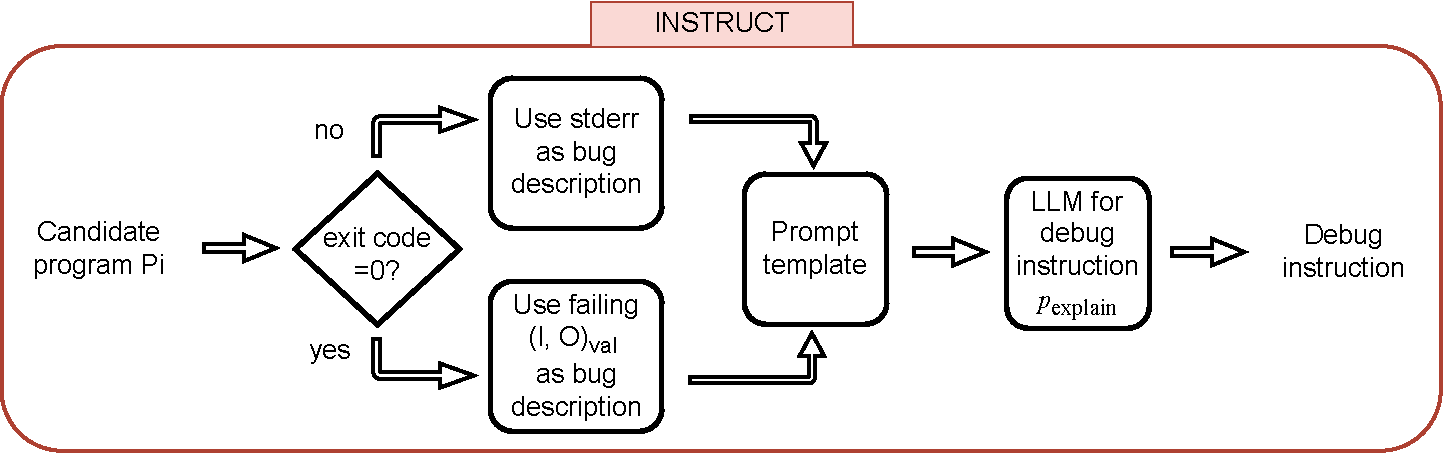
\includegraphics[width=.8\linewidth,trim={0mm 6mm 0mm 0mm}]{codex-for-psb-seidr-instruct-1.drawio.pdf}
    \caption{\instruct{} agent.}
    \label{fig:method-instruct}
    \vspace*{-3ex}
\end{figure*}

\begin{comment}
We consider two different designs of the instruction generation block: \instructs{} and \instructllm{} shown in figure~\ref{fig:method-instruct}. 
Both types of blocks use failing I/O pairs from the validation set and \texttt{stderr} output of the candidate execution. 
In both blocks, if \texttt{stderr} is not empty, i.e., execution errors occur before getting the output to compare it with the expected output, the \texttt{stderr}-based template engine generates an instruction to fix the error mentioned in \texttt{stderr}. 
However, the blocks differ in the way they transform failing I/O pairs to generate instructions in case \texttt{stderr} is empty.

\instructs{} uses a fixed input template and substitutes placeholders for input and output with the corresponding strings of the first failing test case.
We show the resulting instruction for an exemplar template in figure~\ref{fig:method-instruct}.
By contrast, \instructllm{} uses the failing I/O pair in the LLM for text completion, thereby prompting the text LLM to produce the bug summary. 
An exemplar output of the code behavior template engine in figure~\ref{fig:method-instruct} describes that the code returns output O instead of expected output O$_{\text{val}}$ for the failing test case with input string I$_{\text{val}}.$
The LLM is then prompted to auto-complete this description of program behavior with the bug summary. 
The bug description is passed further to the next template engine and used as the debugging instruction, such as ``\emph{Fix~\{bug summary\}}''.
\end{comment}

\paragraph{Debug}

The main component of \method{} which addresses the "near miss syndrome" is the \debug{} agent.  
This agent iterates over all programs in the population to repair the candidate programs and pass more tests. 
It uses the instructions written by \instruct{} to sample from \debugmodel{} model $\treearitydebug{}$ times
to repair every candidate and create a new population of \treearity{} candidates.
For \debugmodel{}, the parameter \texttt{code} is set to the current version of the candidate solution and \texttt{descr} to the output of \instruct{} and any additional context chosen for a specific implementation.
The current generation of candidates is then replaced with \treearity{} outputs of \debug{}.

\paragraph{Rank}

The \rank{} agent implements what is known in genetic programming as \emph{parent selection}~\cite{koza1994:genetic}: it selects the best $\beamwidth{}$ programs to be further improved by the \debug{} agent.
We consider 2 different parent selection algorithms: simple ranking and lexicase selection.

\emph{Simple ranking} sorts the programs by their average test score and selects top $\beamwidth{}$ candidates. 
Such ranking approach is a \emph{quality-based} selection method.
The programs are selected based on the intuition that repair of the best so far (but imperfect) programs begets good programs.

\emph{Lexicase selection}~\cite{helmuth2015:solving} is an approach from the \emph{quality diversity} family that maximizes diversity of selected candidates in addition to their score.
Lexicase selection ensures diversity by keeping the program candidates which perform the best on unique tests as opposed to the program candidates that perform best on average on all tests but, possibly, do not perform perfectly on any unique test.
The algorithm is as follows:
\begin{enumerate}
    \item randomly shuffle the set of tests;
    \item select a program with the best score on test 1;
    \item if several programs are tied, resolve the tie by selecting the best program on test 2;
    \item repeat for tests $3,4,\dots,$ until only one program is left;
    \item mark this program as "selected";
    \item if less than $\beamwidth$ programs are selected, go back to step 1.
\end{enumerate}
This ensures that even if the average quality of selected candidates is lower, the batch of $\beamwidth{}$ programs collectively contains a higher number of requisite "skills", as measured by tests.

See section~\ref{sec:lexicase-results} for their empirical comparison.

\newpage \subsection{Meaning of Hyperparameters}
\label{sec:beam-search}
\begin{figure}
    \centering
    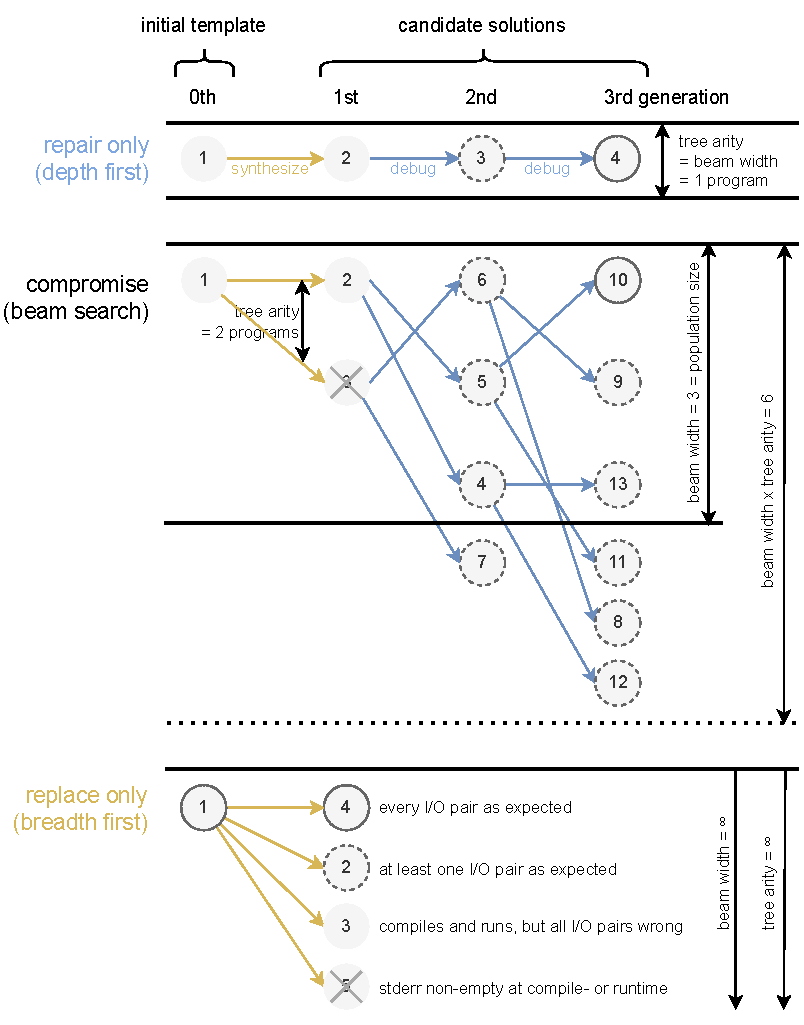
\includegraphics[width=0.6\linewidth, trim={0mm 4mm 0mm 0mm}]{beamsearch.pdf}
    \caption{Repair-replace trade-off as a tree search problem.}
    \label{fig:beam-search}
    % \vspace*{-4ex}
\end{figure}

After evaluating a given candidate solution in \execute{}, \method{} supports two approaches to addressing the candidate's flaws:
\begin{itemize}
  \item \emph{Replace} the candidate with another sample from the current population.
  \item Use \instruct{} and \debug{} to repair the candidate.
\end{itemize}
We refer to this problem as the \emph{repair-replace trade-off}, by analogy with production economics~\cite{jack2000:optimal}. 

How does the choice of hyperparameters $\treearity{},$ the total number of candidate programs in each generation, and $\beamwidth{},$ the number of selected repairs to be preserved in a generation, influence the flow of \method{}?
$\treearity$ and $\beamwidth{}$ act as upper bounds on the \emph{replace} option by limiting the size of the population.
In the edge cases, $\treearity{} = \beamwidth{} = 1$ corresponds to a repair-only process, while $\treearity{} = \beamwidth{} = \infty$ corresponds to replace-only, as illustrated in figure~\ref{fig:beam-search}. 
Note that $\treearity{}$ is defined by $\treearitydraft{}$ for the initial draft solutions in the first generation and $\treearityexplain{} \cdot \treearitydebug{}$ for later generations. 

Observe that a mutation-only genetic algorithm with population size $\beamwidth{},$ such as \method{}, is equivalent to \emph{local beam search} with beam width $\beamwidth{}$ on an $\treearity{}$-ary tree ~\cite[Section 4.1.4]{russell2010:artificial}. This corresponds to a known property of local beam search: it degenerates into depth-first search when $\beamwidth{} = 1$, whereas setting $\beamwidth{} = \infty$ yields breadth-first search.

% Hence, we refer to $\treearity{}$ as \emph{tree arity} and $\beamwidth{}$ as \emph{beam width}.

\newpage \section{Related Work}
\label{sec:related-work}

Until recently, the tasks of program synthesis \cite{gulwaniProgramSynthesis2017} and program repair \cite{gouesAutomatedProgramRepair2019, petke2018:genetic} have been considered separately.
However, a number of important studies bridging this gap in the application of Large Language Models have been carried out concurrently with this work, listed below.

\cite{fanAutomatedRepairPrograms2023} incorporate a program repair step into a program synthesis pipeline where the initial synthesis is done by the Codex model \cite{chenEvaluatingLargeLanguage2021} and for program repair both Codex and state of the art specialized repair tools such as TBar and Recoder \cite{Defects4JDatabaseExisting} are considered and compared. \cite{zhangSelfEditFaultAwareCode2023} do the same, but fine-tune PyCodeGPT-110M \cite{zanCERTContinualPretraining2022} to use it as a repair model. The resulting framework is a two-step process (1 draft step and 1 debug step), while iterative evolution and search are not explored. 

Evolution through Large Models (ELM) \cite{lehmanEvolutionLargeModels2022} proposes using a language model in place of a mutation operator within a traditional genetic programming framework \cite{koza1994:genetic}. They use an type of instruction fine-tuned model trained on git commit messages known as a diff model \cite{DiffModelsNew2023}. However, the model is not directed to solve the programming problem at hand nor to fix bugs, instead, it is provided with generic instructions such as "Change function f". This approach is meant for fields where creative open-endedness~\cite{stanleyWhyGreatnessCannot2015a}, rather then satisfying concrete requirements, is encouraged.

\cite{dongSelfcollaborationCodeGeneration2023} are guided by the metaphor of a multi-agent conversation: their program synthesis loop begins with an analyst LLM generating a plan in natural language, a coder LLM executing it and a tester LLM giving feedback. They implement a repair-only approach and their \execute{} agent is a language model that predicts the output of a program without compilation and/or execution - an instance of chain-of-thought prompting \cite{yuBetterChainofThoughtPrompting2023} for program synthesis.

\cite{jiangSelfEvolveCodeEvolution2023} is a repair-only version of SEIDR that demonstrates the benefits of LLMs evolving not just the source code, but an additional natural language text file that acts as the system's knowledge base, to be included in the model prompt when generating code.

\cite{xiaConversationalAutomatedProgram2023,chenTeachingLargeLanguage2023,shinnReflexionLanguageAgents2023} explore an iterative approach to program synthesis not unlike SEIDR. However, they do not explore the repair-replace tradeoff and exclusively implement the repair-only approach that is prone to local minima.

Finally, Self-Taught Optimizer (STOP) \cite{zelikmanSelfTaughtOptimizerSTOP2023} takes the concept of self-improvement to the next (delightfully meta) level and uses a large language model to edit the evolutionary algorithm itself (i.e. fig. \ref{fig:method}). See their section 8 for reflections on AI Safety.

\newpage \section{Expermental Setup}
\label{sec:eval}

To explore the capabilities of \method{} and its generalisability, we test the framework on two benchmarks  with varied search strategies and use two programming languages. 
The problems in the benchmarks originate from coding competitions and human-written programming assignments. 
During our empirical evaluation of \method{} performance, we address the following research questions:
\head{RQ1. Repair-replace trade-off exploration} 
What is the impact of using different tree search strategies
in the autonomous programming setting? 
We experiment with six different tree arities for the quality-based ranking and study their impact on the number of resolved problems as well as the speed of obtaining solutions.
\head{RQ2. Quality-diversity vs. average quality-first based ranking} 
How does the quality-diversity ranking strategy impact the performance in comparison to average quality-first ranking strategy? 
We run experiments with lexicase selection as the ranking strategy and four non-corner case tree arities.
\head{RQ3. Generalisability of the approach to different LLMs} 
How does the choice of an LLM affect the performance of SEIDR? 
We choose the best performing combination of hyperparameters, i.e., a tree arity and a ranking strategy, for experiments with other LLMs and compare the results with previous work obtained without \method{}. 


\newpage \subsection{Data}
\label{sec:data}

Our experiments use the Program Synthesis Benchmark~2 (PSB2)~\cite{helmuth2022:applying} and HumanEval-X~\cite{zheng2023:codegeex} in C++ and Python. 
The key criteria for the benchmarks choice are availability task descriptions in English and unit tests in Python and C++ or language-agnostic unit tests. 
We focus on the widely used benchmarks in the areas of generative LLMs and genetic programming. 

\paragraph{PSB2}
The first dataset is a benchmark suite of 25 problems for program synthesis that resemble small real-world tasks. PSB2 was developed as a more realistic and challenging version of PSB1~\cite{helmuth2015:general}, the latter consisting of textbook problems and is widely used in genetic programming~\cite{sobania2022:choose}. 
The problems require different data structures and control flows to be used for effective solutions and are taken from sources, such as competitive programming platforms and educational courses. 
The problems have descriptions in English, as well as 1 million~(M) tests for training and 1M testing-stage tests, including edge or corner cases that test the resulting program on complicated inputs. 
The tests are provided as I/O pairs and are distributed together with the problem descriptions as a PyPI package.\footnote{~\url{https://pypi.org/project/psb2/}} 

In PSB1, the training set consists of the edge test cases and is augmented by random test cases if the number of edge tests is not enough. The test set is formed by random test cases. 
This terminology is preserved in PSB2. 
However, we do not have a training or fine-tuning phase in our experiments, because the models are not made available for further training. Instead, we validate the framework with an existing pre-trained LLM for code and text as its parts. 
Therefore, we only have the validation and test phases. 
We will refer to training test cases in the PSB terminology as validation test cases in this study. 

\paragraph{HumanEval-X}
The second dataset we use is a development from the original set of human-written programming tasks in HumanEval~\cite{chenEvaluatingLargeLanguage2021}, which a standard code generation benchmark for LLMs.
HumanEval consists of 164 problems with a docstring representing problem description, a function signature, a correct solution and unit tests in Python. 
HumanEval-X is a result of translation of correct programs and unit tests to five programming languages. 
We use HumanEval-Python for experiments in Python to ensure comparison with other models in the setup without \method{}. 
In addition, we test \method{} on the HumanEval-C++ part of HumanEval-X to compare with results obtained on PSB2. %here and in an earlier \method{} study~\cite{liventsev2023:fully}. 

The test functions of HumanEval-X contain all tests in one function. We split the aggregated test functions into separate tests so that the \rank{} agent can evaluate the \text{score}. 
On average, the number of tests in HumanEval-Python is 7.25 and 6.95 in HumanEval-C++, which is appointed to a repeated additional test present in some HumanEval-Python examples of the following type: \texttt{assert True, "This prints if this assert fails 1 (good for debugging!)"}.
This test type is not present in HumanEval-C++.
To reiterate, we keep the original HumanEval-Python setup for direct comparison with models tested on this benchmark without \method{}. 
Because of the limited number of tests, we pass up to five tests to the draft prompt and make all tests visible to \method{} for the debugging loop. 
In other words, we do not have a held-out test split for HumanEval-X in the same manner as we have it for PSB2.


\newpage \subsection{Models}
\label{sec:models}

\method{} uses three LLMs, \synthmodel{}, \textmodel{}, and \debugmodel{} in \synthesize{}, \instruct{}, and \debug{}, correspondingly. 
These models can be instantiated with the same LLM or different ones. 
The main pre-requisite is that \synthmodel{} and \debug{} are a text-to-code models which take both a textual description and a draft code as input.
Therefore, \synthmodel{} and \debug{} can be a chat model, a code completion model, an instruction fine-tuned or a foundation generative language model pre-trained on code in addition to text. 
By analogy, the text-to-text \textmodel{} can be a chat, instruction fine-tuned, a text completion or generation model pre-trained on text and code.
In our experiments, all three models are instantiated with the same fixed model. 

We use the OpenAI Generative Pre-trained Transformer \texttt{gpt-3.5-turbo}\footnote{\url{https://platform.openai.com/docs/model-index-for-researchers}}  for the experiments with repair-replace trade-off exploration (RQ1) and experiments with quality-diversity and average quality-first ranking strategies (RQ2). 
The GPT-3.5 model is an improvement over the GPT-3~\cite{brown2020:language} 175B-parameter model optimized for chat available via an API.
GPT models are auto-regressive transformer models which have the decoder-only architecture as opposed to the original full encoder-decoder transformer.
They are pre-trained on both text and code and excel at sequence-to-sequence generative tasks, including code-to-code, text-to-code, and code-to-text.

To evaluate generalization capabilities of \method{} on the chosen benchmarks, we have chosen an open-source competitor of GPT models, Code Llama Instruct 34B~\cite{roziereCodeLlamaOpen2023}. 
This model is an advancement on the Llama 2 model~\cite{touvron2023:llama}, an auto-regressive transformer model fine-tuned for code infilling (cloze-style generation), processing longer context windows and instructions.
This model is run as an with the best performing set of hyperparameters found for GPT-3.5 on each of the benchmarks in C++ and Python.
We also compare the performance of \method{} with the current state-of-the-art without \method{} as reported in the corresponding studies (see Section~\ref{sec:results-rq3}).

\newpage \subsection{Prompts}
\label{sec:prompts}

Our implementation is optimized for instruction and chat models, which use prompts as inputs represented as text, partially with code fragments.
The models use a system message which describes the ``role'' of the LLM and a regular message that works as an instruction or a chat message from a user.
To provide more context, we always use a problem description, problem name, programming language to the model as textual input (\texttt{descr}). 
As code, we also add an initial template depicted in figure~\ref{fig:template} to \synthmodel{} and the current program candidate to \textmodel{} and \debugmodel{}.

The resulting prompts are as follows.
System message is: 

\begin{lstlisting}
You are an experienced software developer. You write concise code in \{language\}.
The code must read input from user and return output corresponding to the task description.
\end{lstlisting}

Input to \synthmodel{} looks as follows:

\begin{lstlisting}
Solve the following code contest problem: \{problem\_name\}. 
Problem description: \{problem\_description\}.
\{program\_template\}
Only complete the code, do not add triple quotes, do not give explanations.
\end{lstlisting}

Bug explanations are generated with \textmodel{} using the following instructions:

\begin{lstlisting}
  I'm trying to solve the following code contest problem: \{problem\_name\}. 
Problem description: \{problem\_description\}.
Currently, the code is 
\`{}\`{}\`{}
\{program\_candidate\}
\`{}\`{}\`{}
The issue is 
\{stderr or "it must return \{expected\_output\} for input \{input\}, but it returns \{output\}".
Describe how I should fix the code in a very concise manner.
\end{lstlisting}

Debugging model \debugmodel{} operates on the following instruction:

\begin{lstlisting}
Solve the following code contest problem: \{problem\_name\}.
Problem description: \{problem\_description\}.
Currently, the code is 
\`{}\`{}\`{}
\{program\_candidate\}
\`{}\`{}\`{}.
Modify the code as \{bug\_summary\}.
You must only return correct code. Remove any triple quotes, language name or explanations.
\end{lstlisting}


\newpage \subsection{Repair-replace Trade-off Settings}
\label{sec:trade-off-settings}

As described in Section~\ref{sec:beam-search}, the choice of beam width $\beamwidth{}$ and tree arity $\treearity{}$ define the repair-replace trade-off where higher $\beamwidth{}$ and $\treearity{}$ prioritize to repair over replace. 
In the meantime, each of the three LLMs can generate sequences in batches. 
We generate $\treearitydraft{}$ programs in the first generation with \synthmodel{}, $\treearityexplain{}$ bug explanations with \textmodel{} for each program in the first generation, and $\treearitydebug{}$ candidate repairs for each of the debugging instructions using \debugmodel{}.
A new generation of $\treearityexplain{} \cdot \treearitydebug{}$ programs is ranked and filtered to keep the best performing $\beamwidth{}$ candidate programs for generating the next candidates. 

To balance between a reasonable number of experiments and diverse sets of hyperparameters, we fix $\treearityexplain{}=2$ to moderately vary the bug descriptions and set $\treearitydraft{} = \treearitydebug{}.$
The upper limit for the total number of generated program candidates is set to 100 to limit the experimentation time. 
We evaluate six options for these hyperparameters as shown in table~\ref{tab:w-n} in the experiments with average quality-first ranking and four non-corner case options for quality-diversity ranking with lexicase selection. 
The choice of these tree branching hyperparameters and the maximum number of generated programs is motivated by the earlier study, where the best results were obtained for $\treearity{}=10,$ so we explore the area around this value more closely.
In the same study, the majority of problems in PSB2 were solved within the set of first 100 generated programs. Note that the setting $\treearitydraft{}=\beamwidth{}=\infty$ ensures that a second generation of programs does not exist.

\begin{table}
    \centering
    \caption{Tree search hyperparameters.}\small
    \label{tab:w-n}\vspace*{-4mm}
    \begin{tabular}{rcccccc}
    \toprule
    experiment & 1 & 2 & 3 & 4 & 5 & 6 \\
    \midrule
     beam width, $\beamwidth{}$ & 1 & 4 & 8 & 10 & 16 & $\infty$ (100) \\
     \# programs in the 1st generation, $\treearitydraft{}$ & 1 & 4 & 8 & 10 & 16 & $\infty$ (100) \\
     \# bug explanations for candidate, $\treearityexplain{}$ & 2 & 2 & 2 & 2 & 2 & - \\
     \# repairs for each explanation, $\treearitydebug{}$ & 1 & 4 & 8 & 10 & 16 & - \\
     \midrule
     used in quality-diversity ranking & 
     no & yes & yes & yes & yes & no \\
     used in average quality-first ranking  & 
     yes & yes & yes & yes & yes & yes \\
     \bottomrule
    \end{tabular}
\end{table}



\newpage \subsection{Performance Indicators}
\label{sec:metrics}

\sloppy %
In our experiments, we compare 
the number of fully solved programs obtained using \method{} with different values of hyper-parameters. 
For a more detailed analysis of results, we use \emph{test pass rate (TPR)} and \emph{Excess Programs Generated (EPG)}.
TPR reflects the percentage of fully passed test cases based on the exact match of program output and test output. 
The TPR metric is used for the final evaluation of generated programs and does not reflect partial passing of the I/O test as opposed to the \emph{score} as calculated by the \rank{} agent. 
To compare our results with recent LLMs, we use \emph{pass@k} metric that shows how many problems have $TPR=1$ if we cut off the tree after generating $k$ programs. 

\debug{} and \execute{} agents generate a number of programs that are replaced or repaired during the search for solution program. 
The number of programs generated before the first occurrence of the program that passes all validation test cases is referred to as EPG. 
EPG is indicative of the computational cost of solving a problem distributed in terms of LLM inferences and program compilations and executions.

\newpage \subsection{Implementation Details}
\label{sec:implementation}

To operate with the chosen LLMs in \method{}, we use ollama\footnote{\url{https://ollama.ai/}} and LangChain.\footnote{\url{https://www.langchain.com/}}  
To ensure that the program candidates generated from the same parent program are different from each other, we change the temperature parameter of LLMs. 


Due to repetitive calls to \execute{}, we have to resolve the speed of testing versus precision trade-off while choosing the number of validation test pairs.
We resolve the trade-off by fixing the validation set size at~100. Due to a small number of tests in HumanEval-X, all tests are made visible during the validation step. 
We use 2000 I/O pairs from the test split of PSB2 to evaluate the candidate program that has passed all the validation test cases during debugging. 

In all the experiments, we set the limit to generate a maximum of 100 program candidates during the search of the candidate that passes all validation tests. 
If we reach 100 candidates and none of them passes all validation tests, we report the test pass rate for the last generated candidate. 

\newpage \section{Results and Discussion}
\label{sec:results}

In this section, we present combined results for the replace-repair trade-off and ranking approaches and discuss them in the dedicated sections. 
Specifically, we count the number of fully solved problems or tasks as measured by $TPR=1$ in experiments with the settings described in table~\ref{tab:w-n} and present the language-specific results for PSB2 and HumanEval in the figure below:

\begin{figure}[H]
 %
\begin{subfigure}{\linewidth}
\centering
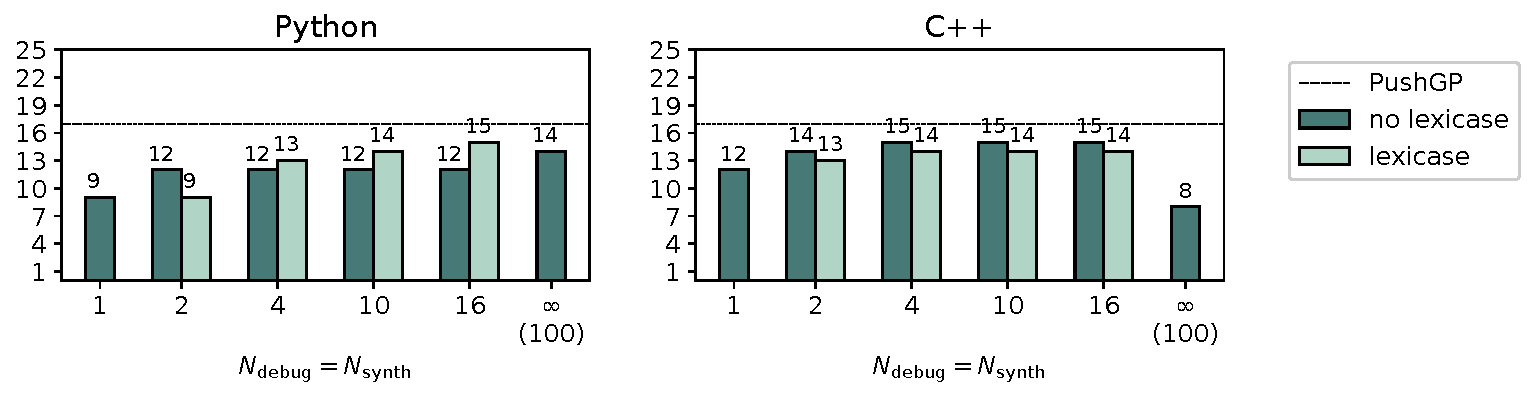
\includegraphics[width=\linewidth, trim={0mm 4mm 0mm 0mm}]{num_solved_problems_vs_bf_psb2_gpt35_01.pdf}
  \caption{PSB2.}
  \label{fig:psb2-gpt3.5}
\end{subfigure}
% \vspace{2mm}
\begin{subfigure}{\columnwidth}
\centering
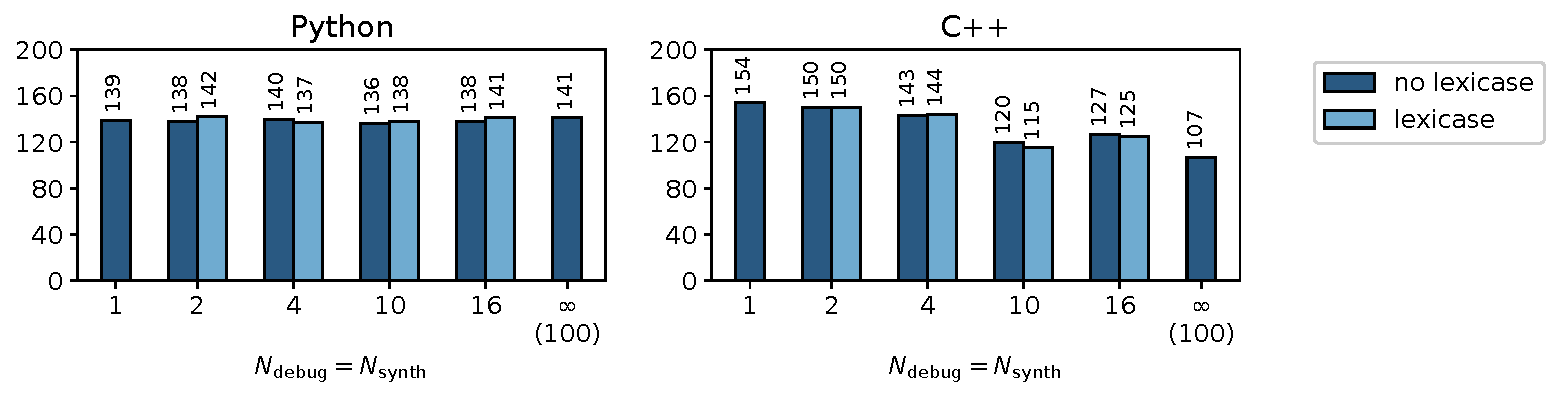
\includegraphics[width=\linewidth, trim={0mm 4mm 0mm 0mm}]{num_solved_problems_vs_bf_humaneval_gpt35_01.pdf}
  \caption{HumanEval}
  \label{fig:he-gpt3.5}
\end{subfigure}
% \vspace{-2mm}
\caption{Repair-replace trade-off with GPT3.5}
\label{fig:repair-replace-trade-off-gpt3.5}

\end{figure}

The figure demonstrates the total number of solved problems as measured by $TPR=1$ using \method{} with GPT-3.5 for the experiments with different numbers of generated programs per instruction ($\treearitydraft$ and $\treearitydebug{}$) and ranking types.

We also explore the speed of obtaining each individual solution with the same experiment settings and report them for PSB2 in figure~\ref{fig:epg-psb2}, HumanEval-Python and HumanEval-C++ in figures~\ref{fig:epg-humaneval-python} and~\ref{fig:epg-humaneval-c++}, correspondingly.
Other experiment-specific graphs and tables are described in the dedicated sections. 


\newpage \subsection{RQ1. Repair-replace Trade-off Exploration}
\label{sec:rq1}

We compare the number of solved problems in the experiments with $\treearitydraft{}=\treearitydebug{}$ values of 1, 2, 4, 10, 16, $\infty$ (100) and $\treearityexplain{}=2$ in Python and C++ in figure~\ref{fig:repair-replace-trade-off-gpt3.5}. 
We will refer to the (equally set) values of $\treearitydraft{}$ and $\treearitydebug{}$ as $N^*$ further in the text.
The results of \method{} are compared to the baseline performance of PushGP on the PSB2 benchmark, which solves 17 out of 25 problems. 
Note that experiments with $N^*=1$ and $N^*=\infty$ can be considered as ablation studies, where the replace option and repair option is turned off, correspondingly. 

For PSB2, the results highlight the benefit of compromise strategies with tree arity of 2, 4, 10, and 16 over repair-only ($N^*=1$) and replace-only ($N^*=\infty$) strategies (see figure~\ref{fig:psb2-gpt3.5}). 
The repair-only scheme is outperformed by other strategies. 
We explain the poor performance of repair-only strategy by the fact that the search space is under-explored. 
Specifically, the replace scenario ensures the LLM for debugging represented by GPT-3.5 in our experiments generates different updates of program candidates using variable temperature.
The probability of finding a better fix is higher when more alternatives are generated to update the draft program at $N^*>1$ compared to $N^*=1$. 
The search strategy with lexicase selection and $N^*=16$ yields the best results on Python and tree arities  $N^*=4, \; 10, \; 16$ with the average quality-first search strategy outperform other tree arities but do not outperform PushGP.
Note that \method{} with Codex (GPT-3 trained on code) as \synthmodel{} and \debugmodel{} and GPT-3 as \textmodel{} does outperform PushGP on Python and performs on par with PushGP in C++ with $N^*=10$ and $\treearityexplain{}=1$. %as described by \cite{liventsev2023:fully}.
This can be explained by the generic chat-tuned nature of GPT-3.5 as opposed to Codex' code-specific pre-training. 
% The results imply that generating a moderate number of programs in parallel during the \debug{} step works better than the policies in which more updates are generated for each program (2-16) or only one program is updated iteratively on the datasets .

For HumanEval-C++, the trend is that the larger number of tasks are solved with smaller tree aritites holds (see figure~\ref{fig:he-gpt3.5}). 
However, the leading tree arity value is $N^*=1,$ which diverges from the PSB2 findings. 
In HumanEval-Python, the best result is obtained with  $N^*=2$ with lexicase selection, while the second best result is observed for $N^*=16$ with lexicase  selection and $N^* = \infty \; (N^*=\text{max programs}=100)$ without lexicase selection.
It is notable that HumanEval-X has less tests than PSB2 which suggests that with more thorough testing, the leading tree arity can be different.

The speed of finding a solution broken down to the problem level is shown in the figures below. Number of Excess Programs Generated are reported in color and test pass rate as numbers depending on the type of debug prompt. Higher EPG values are shown in darker shades than low EPG. We denote solved problems with ``+'' (test pass rate = 1), unsolved problems with ``-'' (test pass rate = 0), and show the test pass rate for partially solved problems.

\begin{figure}[H]
  \centering
  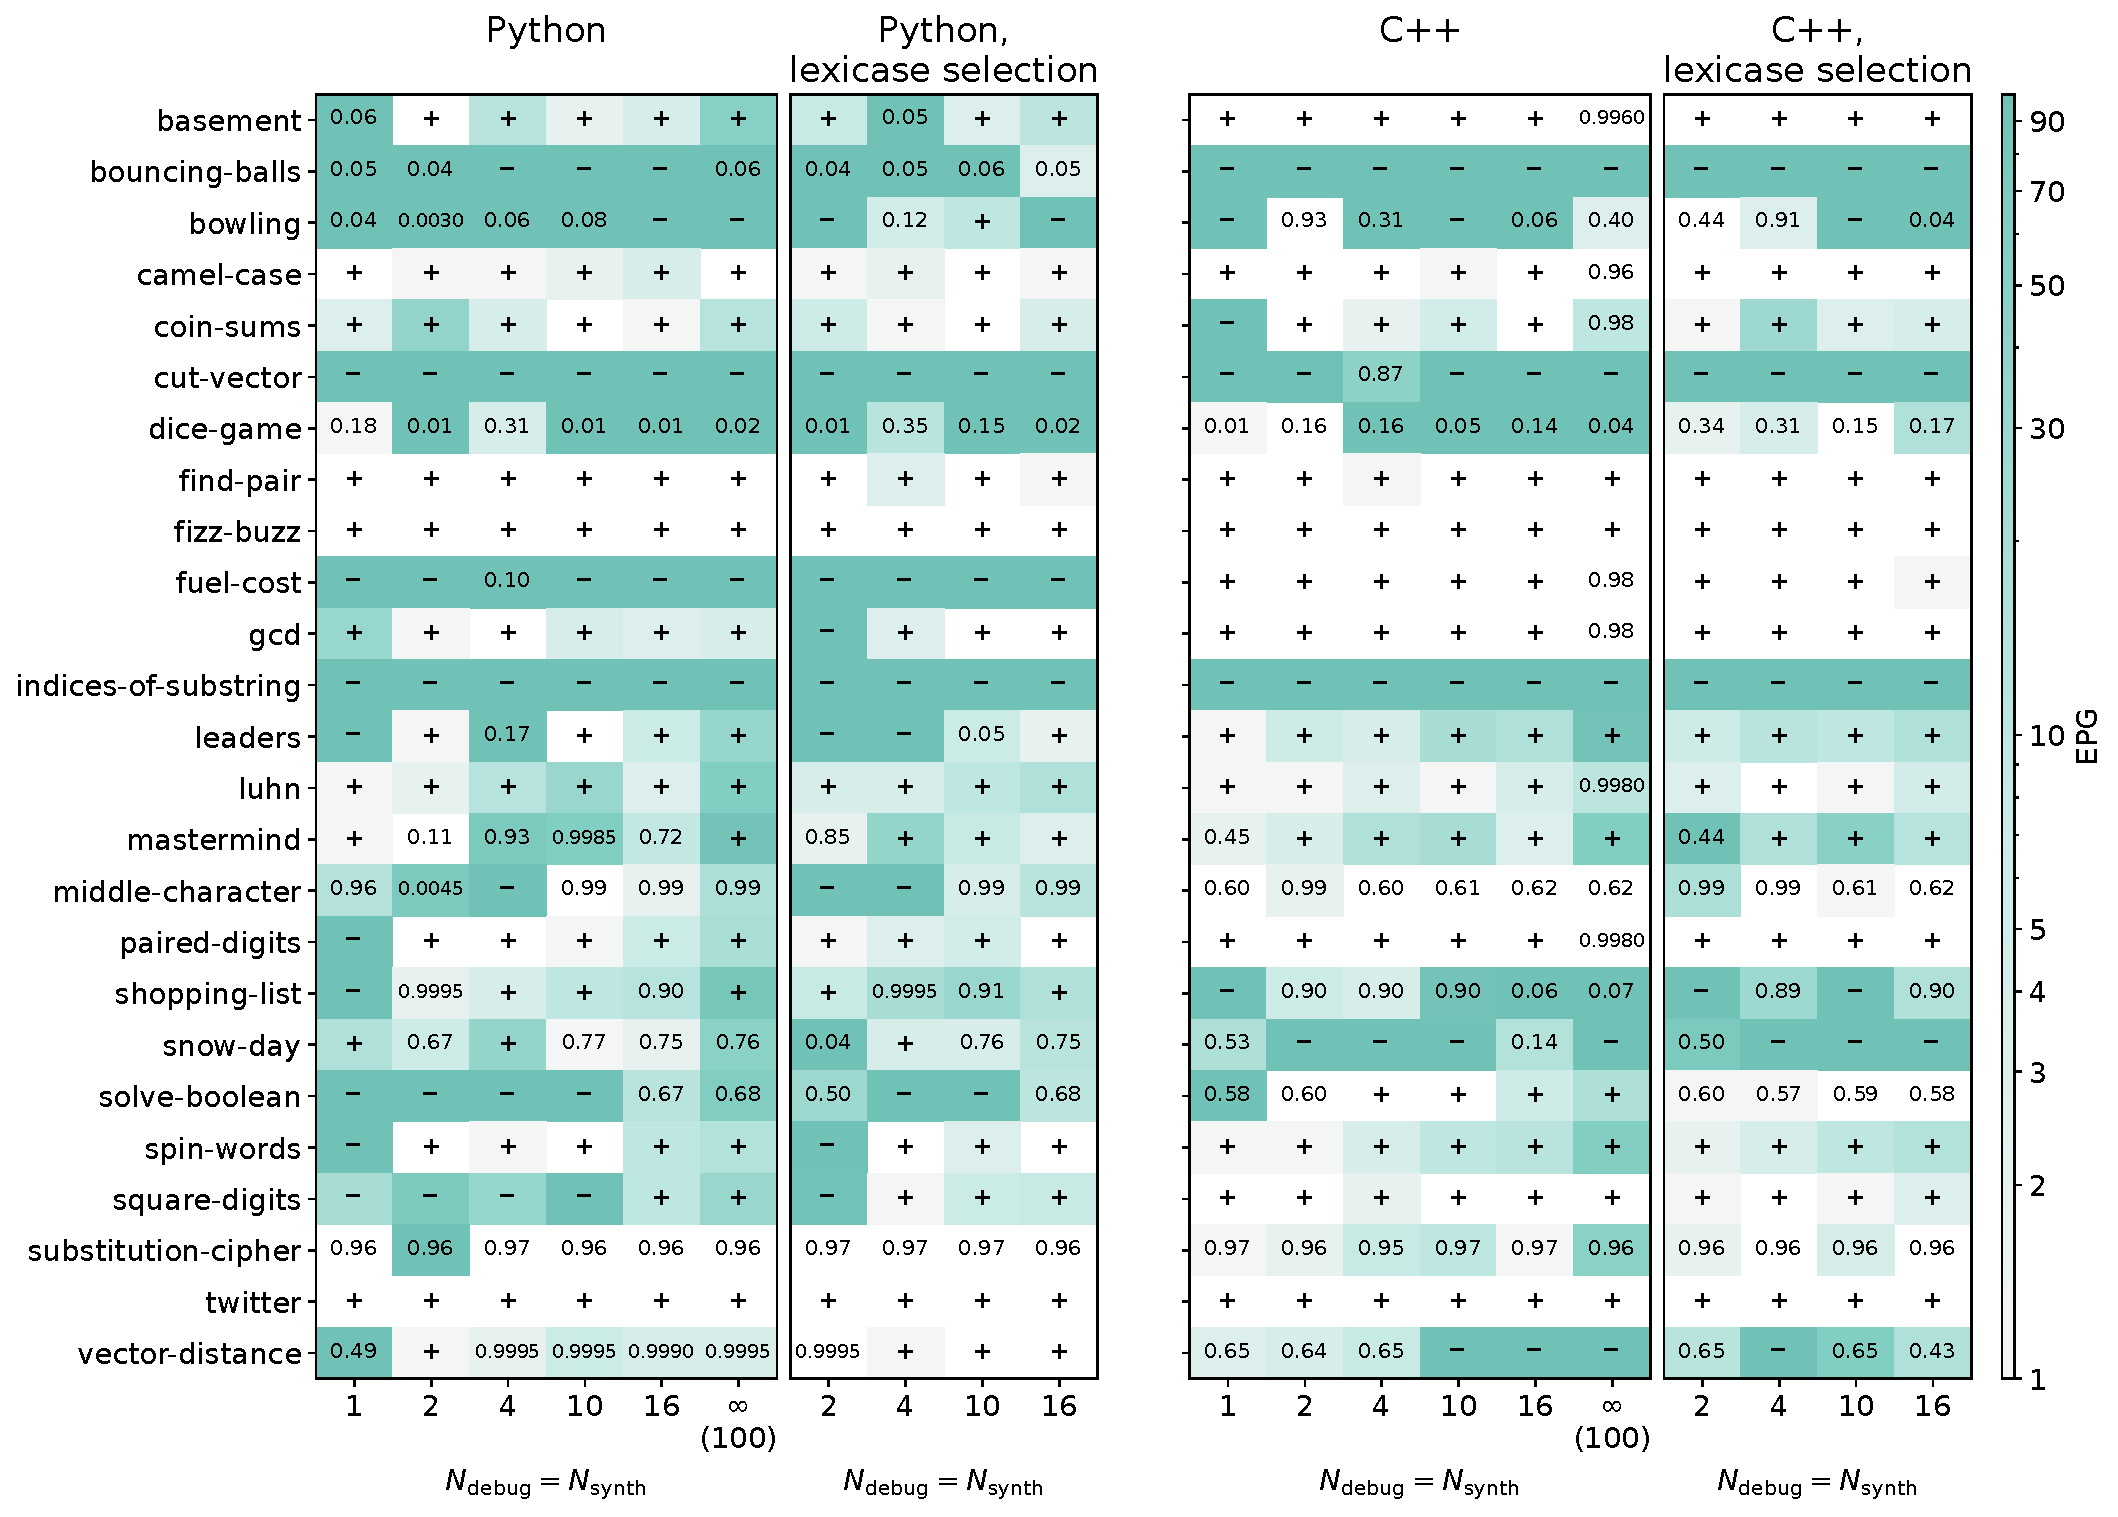
\includegraphics[width=.82\linewidth, trim={0mm 2.8mm 0mm 2mm}, clip]{epg_psb2_gpt35_01.pdf}
  \caption{EPG and Test Pass Rate for PSB2. }
  \label{fig:epg-psb2}
\end{figure}


\begin{figure}[H]
  \centering
  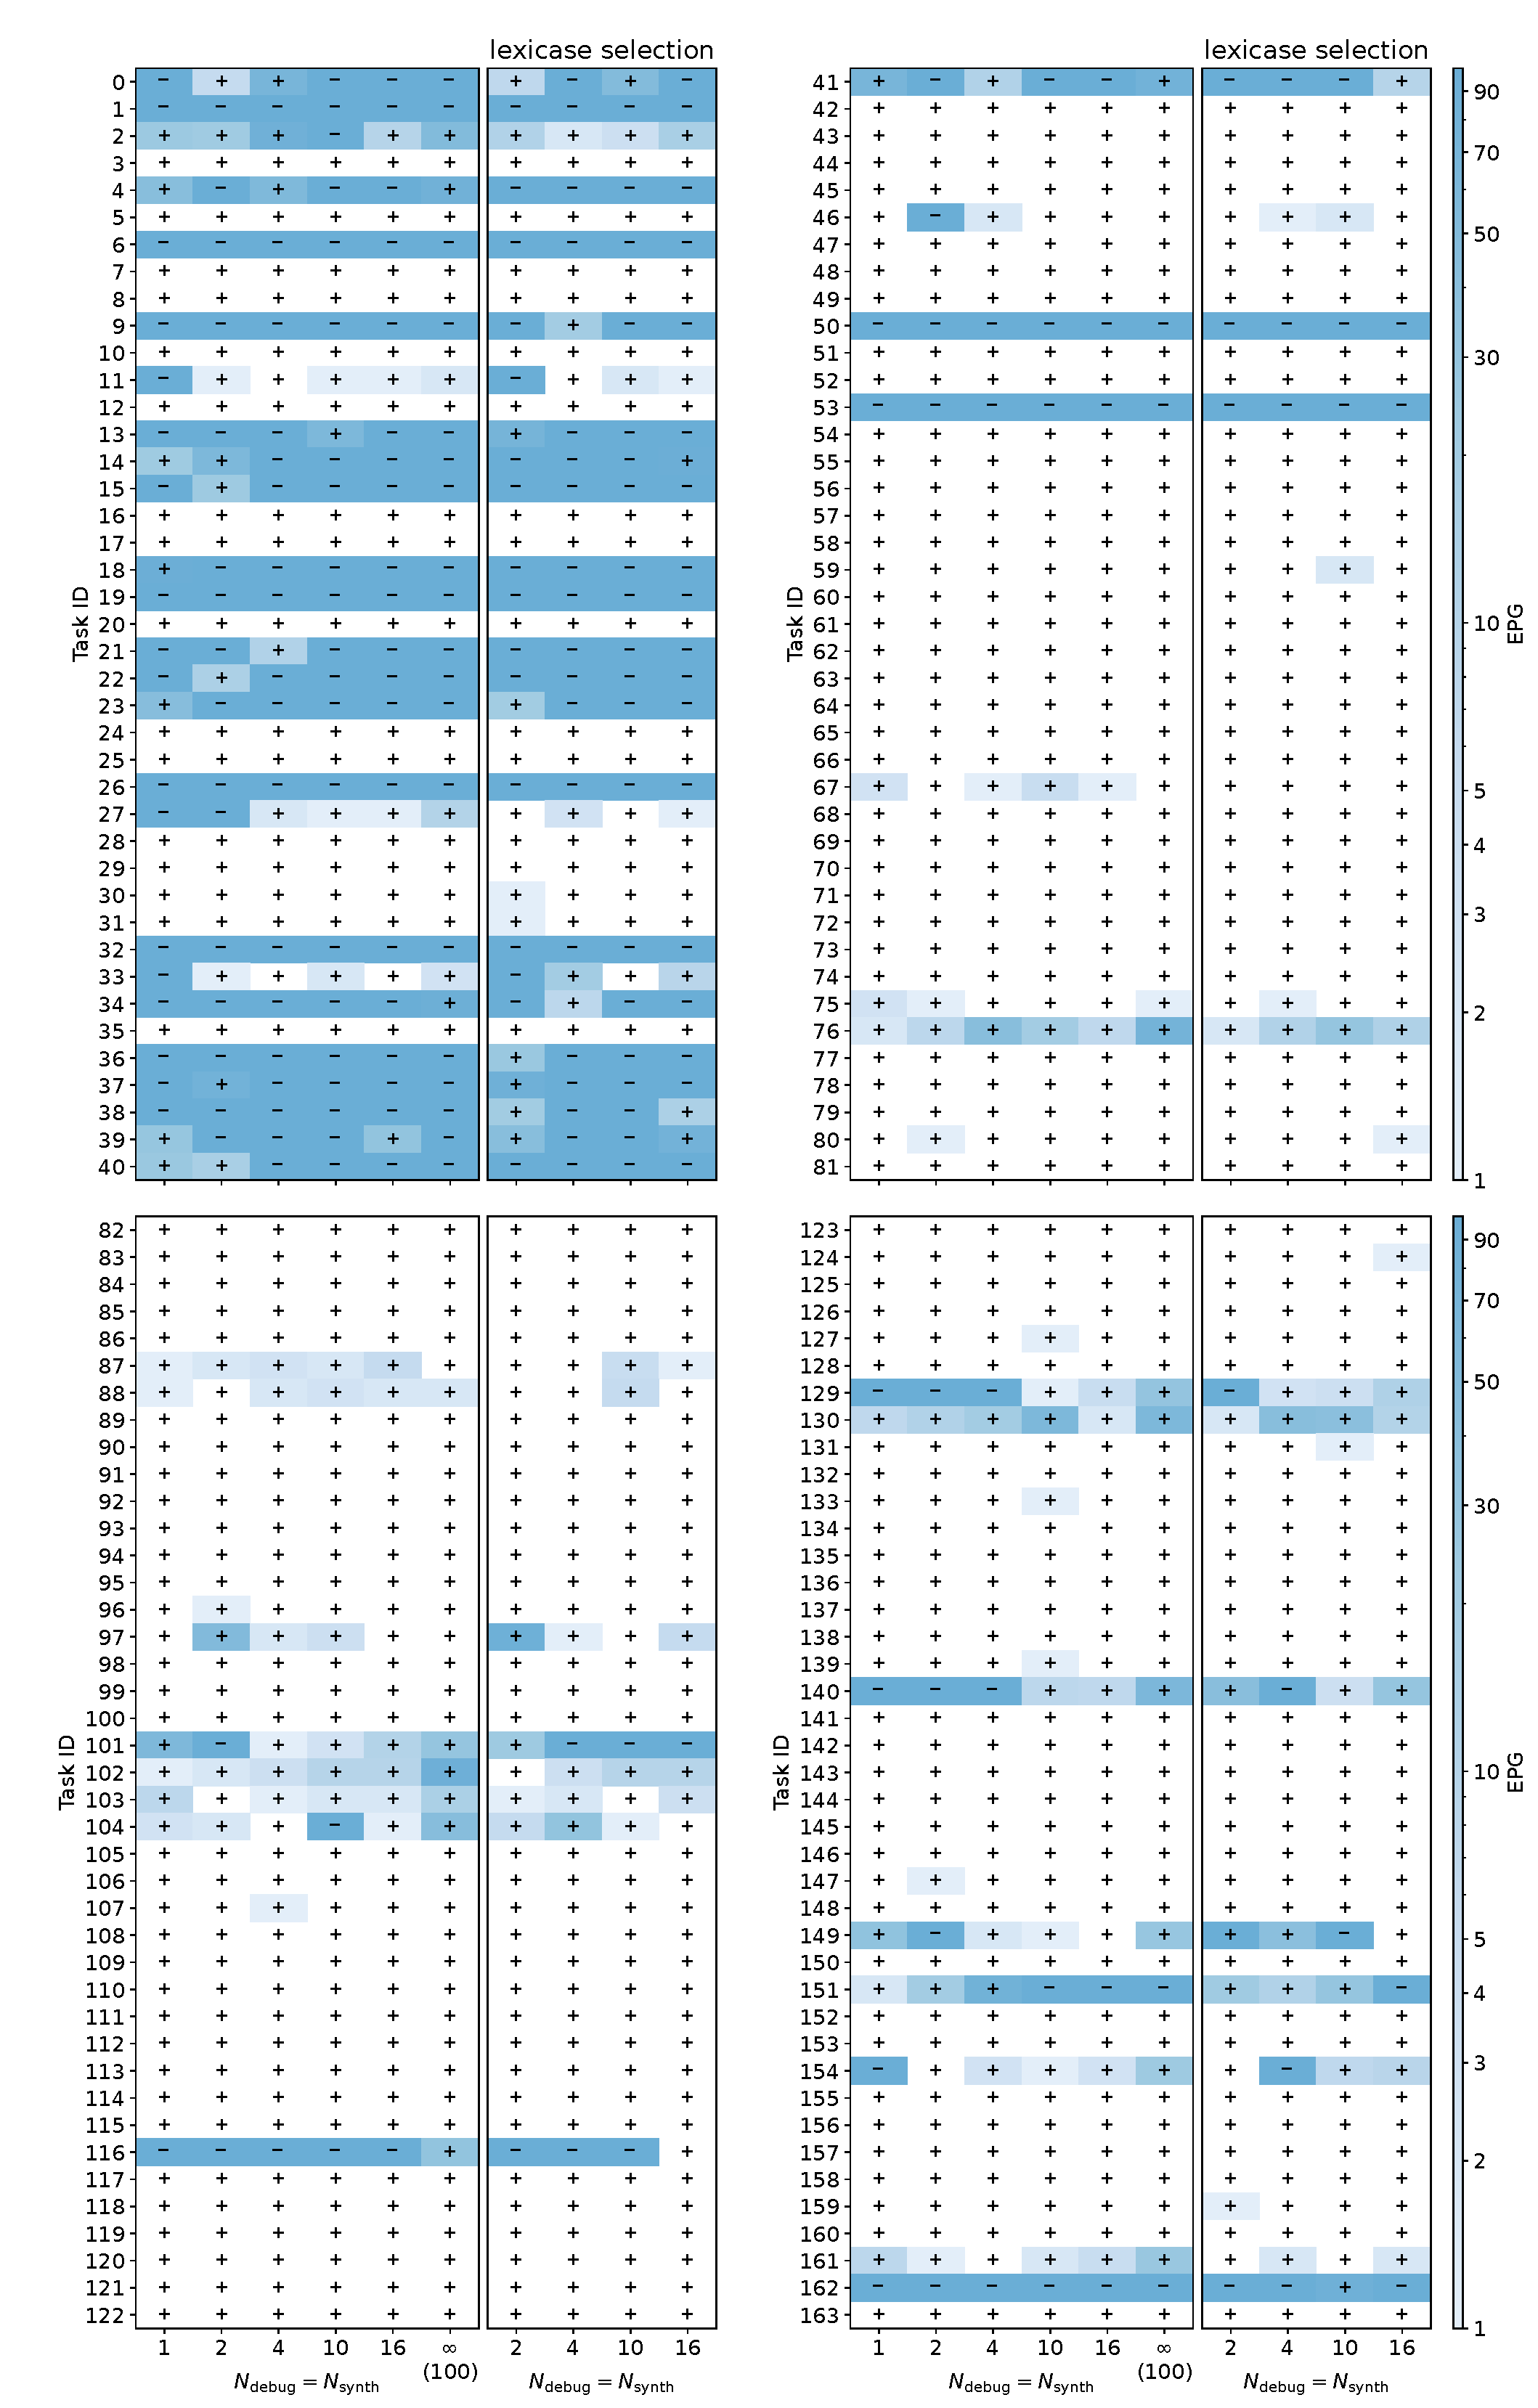
\includegraphics[width=.82\linewidth, trim={0mm 2.8mm 0mm 2mm}, clip]{epg_humaneval_Python_gpt35_01.pdf}
  \caption{HumanEval-Python: Excess Programs Generated and Test Pass Rate.}
  \label{fig:epg-humaneval-python}
\end{figure}

\begin{figure}[H]
  \centering
  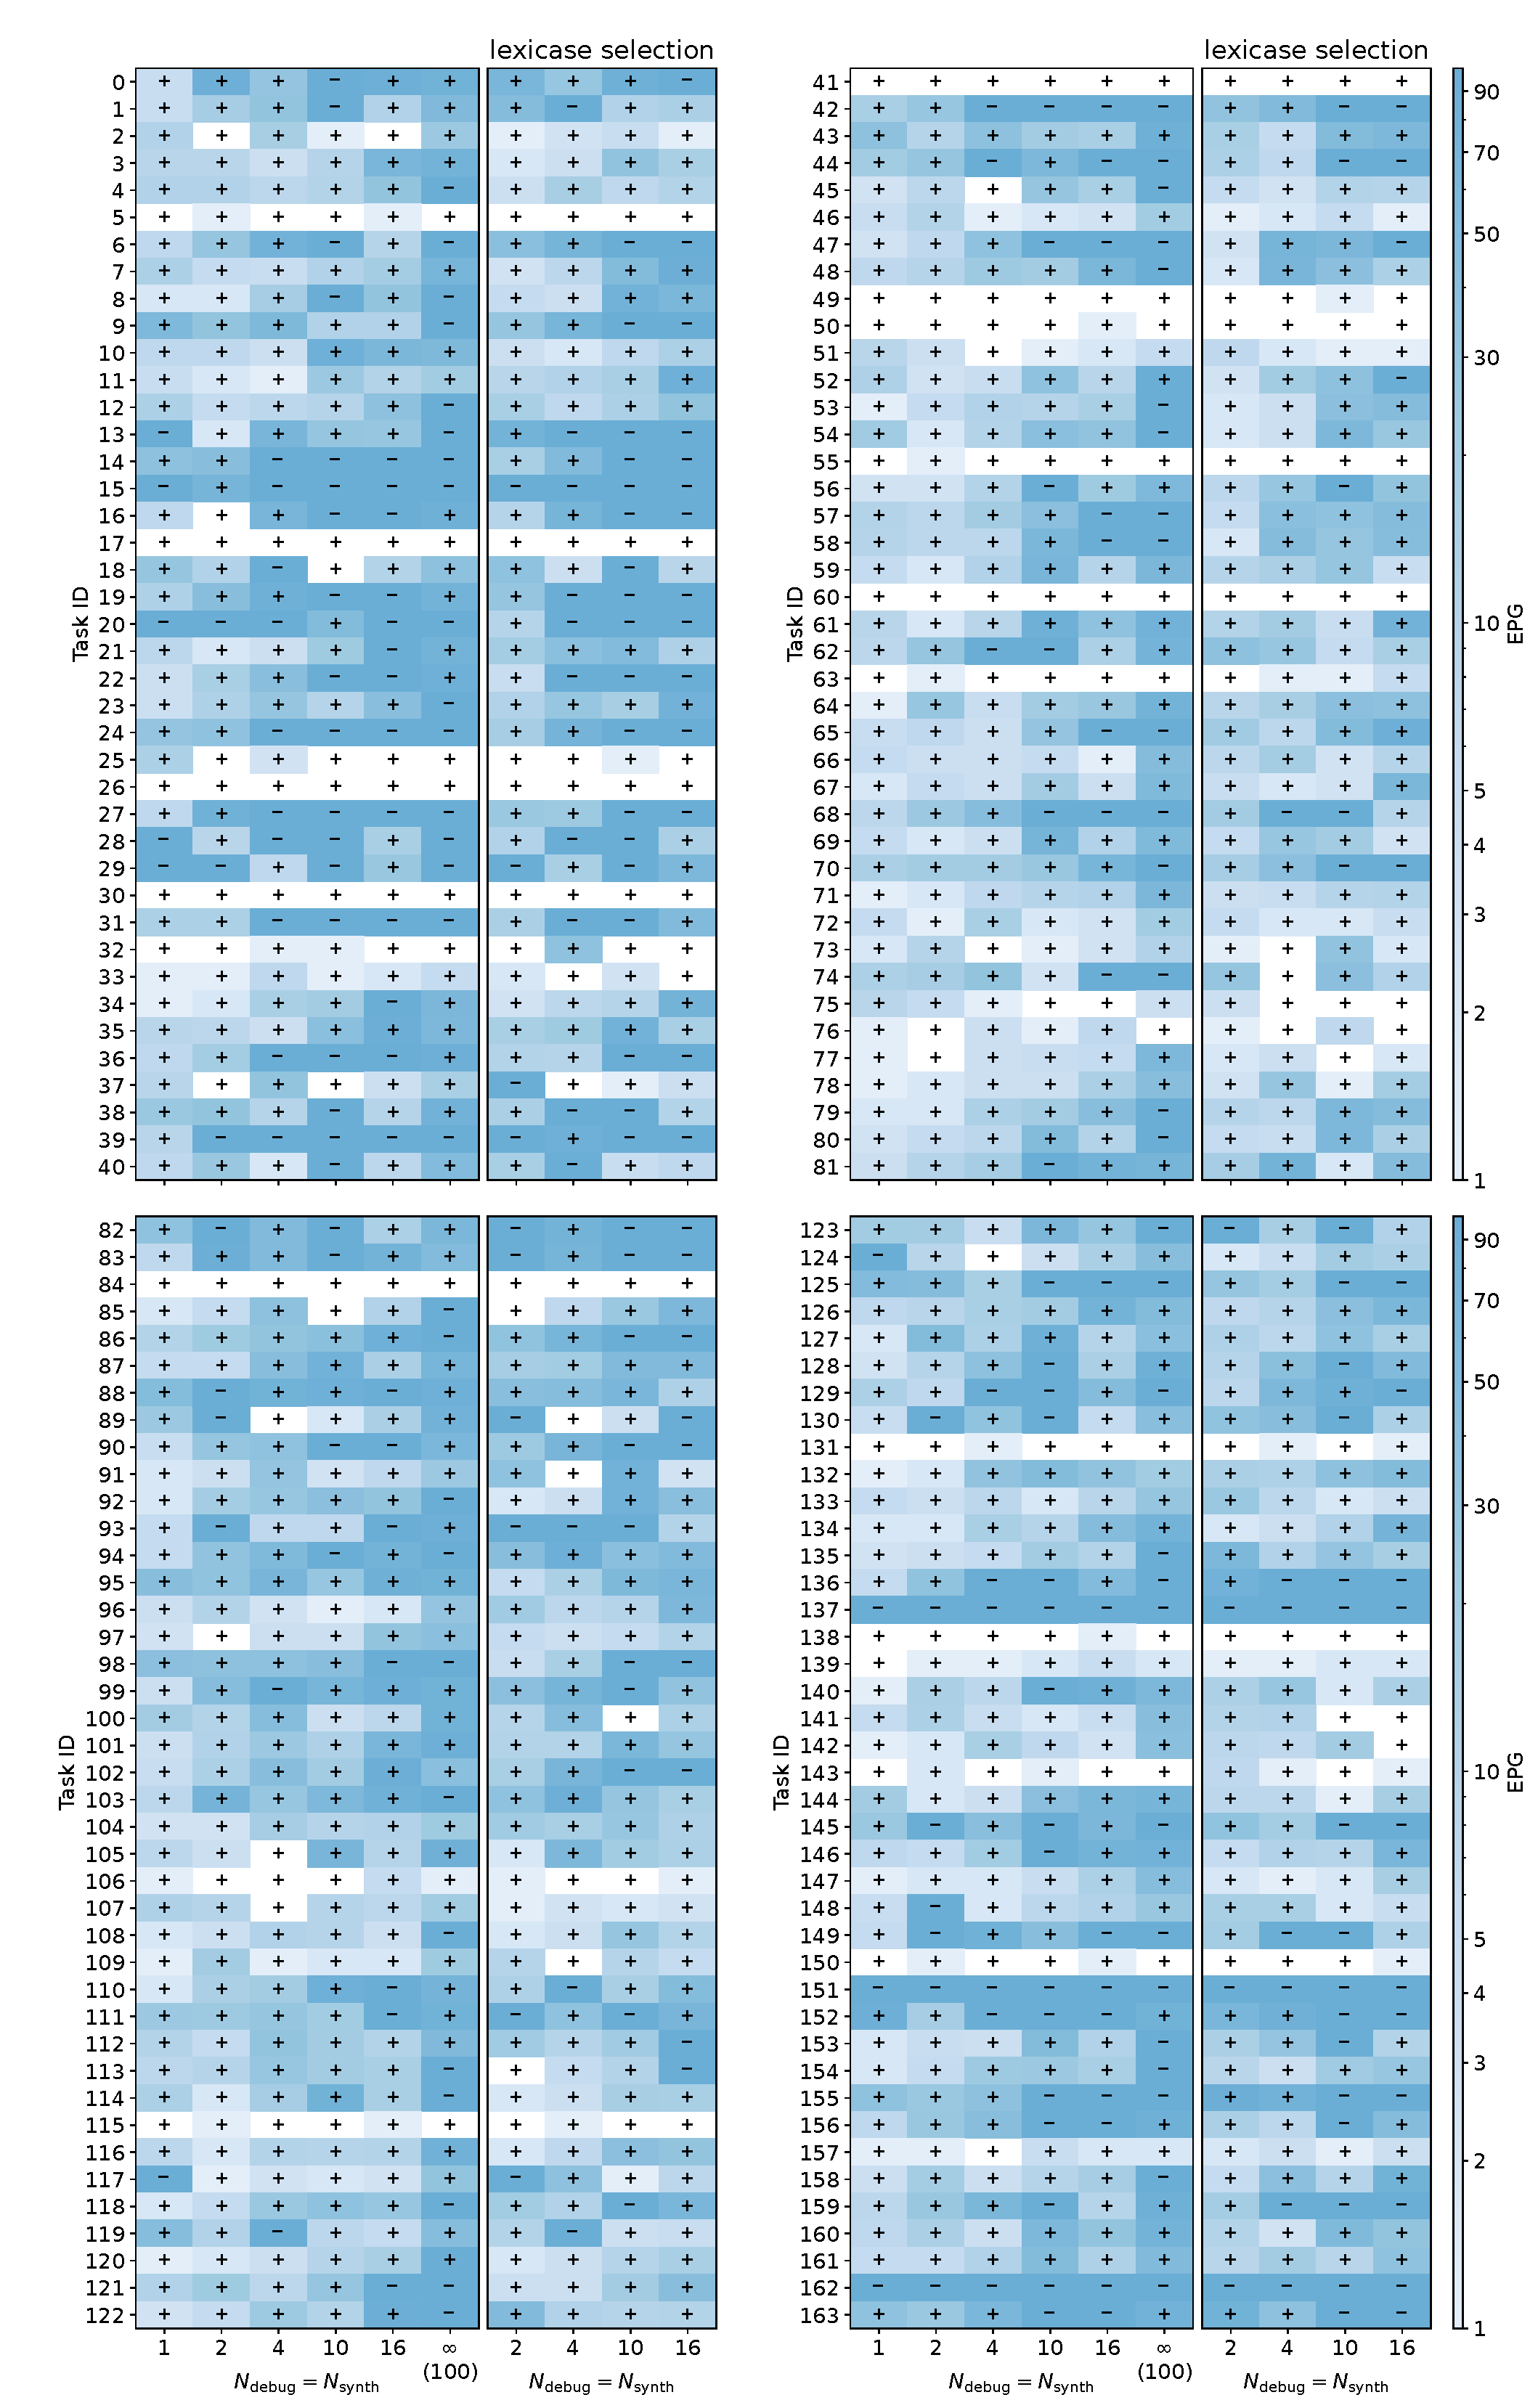
\includegraphics[width=.82\linewidth, trim={0mm 2.8mm 0mm 2mm}, clip]{epg_humaneval_C++_gpt35_01.pdf}  %
  \caption{HumanEval-C++: Excess Programs Generated and Test Pass Rate .}
  \label{fig:epg-humaneval-c++}
\end{figure}

In PSB2, the fastest solutions to all validation sets without lexicase  selection in Python is found using $N^*=16$ (observed in columns with the prevalence of light-colored cells over the dark-colored cells), both with and without lexicase  selection, and in C++  using $N^*=2$, with and without lexicase selection, with a runner-up of $N^*=16$ with lexicase  selection.
Bowling in Python, PSB2, and task 162 in HumanEval-Python experiments are the only problems solved by a unique set of hyperparameters, $N^*=10$ with lexicase selection, and not solved by any other set of hyperparameters.

In HumanEval-Python, for the majority of solved tasks, the solutions are found at the first attempt which negatively influences the analysis of repair-replace trade-off on this dataset, since all tree search algorithms are equivalent when the root node of the tree is the solution.
For HumanEval-Python, task IDs 11, 27, 33, 101-104, 129-130 are solved faster with $N^*=4, \; 10$ with lexicase selection and $N^*=4, \; 10, \; 16$ without lexicase selection more frequently than with other values of $N^*$ (see figure~\ref{fig:epg-humaneval-python}).
The trend of better results with smaller values of $N^*$ is true both for the number of solved problems (figure~\ref{fig:he-gpt3.5}) and higher speed of finding solutions (see figure~\ref{fig:epg-humaneval-c++}) in C++.
% Smaller values of $N^*$ result in both faster and more solutions (without lexicase selection or on par with it) for HumanEval-C++, which is indicated by brighter colors in the columns on the left of the heatmaps compared to the columns on the right.

\begin{highlight}
\textbf{Answer to RQ1:} 
Search strategies in \method{} with tree arity $N^*$ larger than one and lower than $\infty$ benefit from the replace possibility of the \method{} framework as a consequence of using variable temperature for GPT-3.5 on PSB2.
In the experiments, where the majority of problems are solved with more than one attempt, such as HumanEval-C++, lower tree arities (1, 2, 4) yield better results, which indicates the importance of the \debug{} agent in \method{}. 
No single leading tree arity $N^*$ was found for \method{} with GPT-3.5 on PSB2 and HumanEval-X.
\end{highlight}

\newpage \subsection{RQ2. Experimenting with Average Quality-first and Quality-diversity Ranking Strategies}
\label{sec:lexicase-results}

Quality-diversity ranking is implemented as lexicase selection and tested with the number of generated programs in the first generation (drafts) and candidates generated from bug explanations (tree arities $N^*=2,\; 4, \; 10, \; 16$) as mentioned in table~\ref{tab:w-n}.
We have partially discussed the results concerning the use of lexicase selection and average quality-first ranking while describing figures~\ref{fig:repair-replace-trade-off-gpt3.5} and~\ref{fig:epg-psb2}-\ref{fig:epg-humaneval-c++}. 
Therefore, in this section, we focus on the cases where lexicase selection-based ranking outperformed average quality-first ranking and the speed of obtaining solutions with lexicase selection and average quality-based ranking.

We present the analogy of the solution speed metric for all tree arity values and fixed default debug instruction in figure~\ref{fig:epg-distribution}. 
In detail, we show the distribution of EPG values in all experiments to explore how many candidate updates are generated before the solution is found.
We zoom in to the cases with solutions found with up to the first 10 program candidates in figures~\ref{fig:psb2-epg-distrib-step-1} and~\ref{fig:humaneval-epg-distrib-step-1} for PSB2 and HumanEval-X, respectively. 
The coarser-grained EPG distribution with the step of 10 candidates is shown in figures~\ref{fig:psb2-epg-distrib-step-10} and~\ref{fig:humaneval-epg-distrib-step-10}. 

% %%%%%%%%%%%%%%%%%%%%%%%%%%%%%%%%%%%%%%%%%%
% % EPG distribution
% %%%%%%%%%%%%%%%%%%%%%%%%%%%%%%%%%%%%%%%%%%
\begin{figure}
 %
\begin{subfigure}{\columnwidth}
\centering
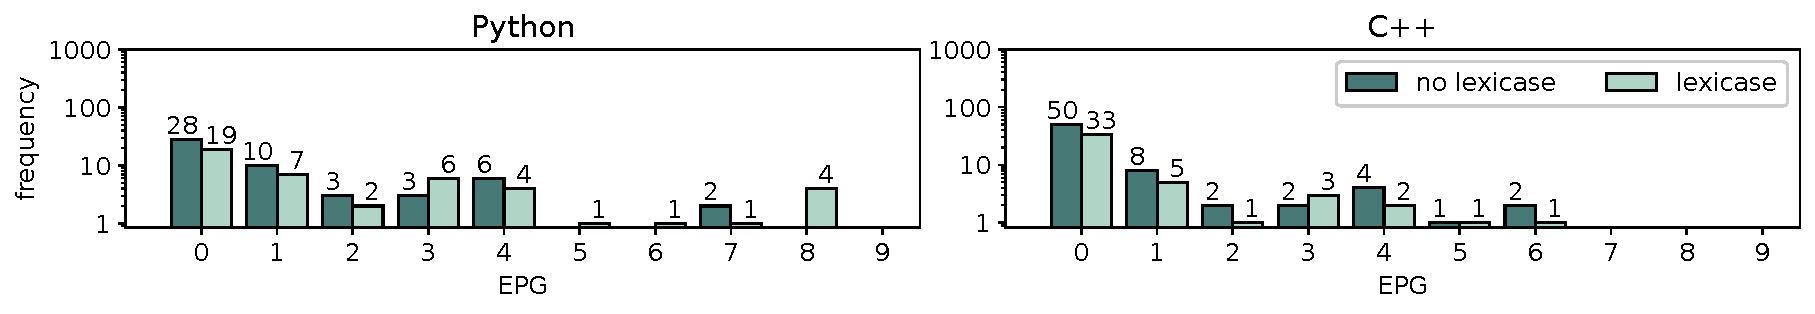
\includegraphics[width=\linewidth, trim={0mm 4mm 0mm 0mm}]{epg_distribution_psb2_gpt35_1_01.pdf}
  \caption{HumanEval: 0 $\leq$ EPG $\leq$ 10 with step 1.}
  \label{fig:psb2-epg-distrib-step-1}
\end{subfigure}
% 
% 
\begin{subfigure}{\columnwidth}
\centering
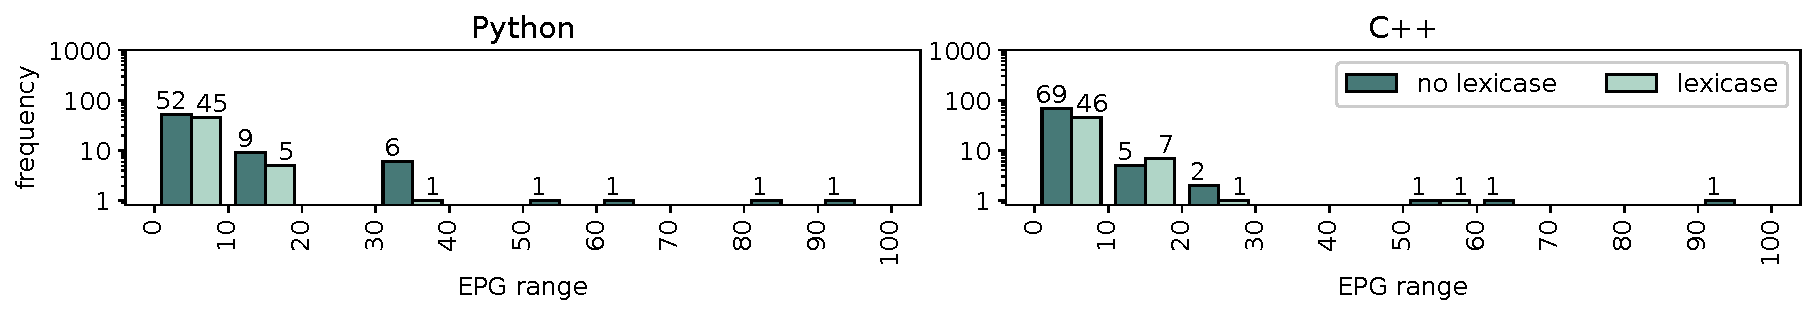
\includegraphics[width=\linewidth, trim={0mm 4mm 0mm 0mm}]{epg_distribution_psb2_gpt35_10_01.pdf}
  \caption{HumanEval: 0 $\leq$ EPG $\leq$ 1000 with step 100.}
  \label{fig:psb2-epg-distrib-step-10}
\end{subfigure}
% 
\begin{subfigure}{\columnwidth}
\centering
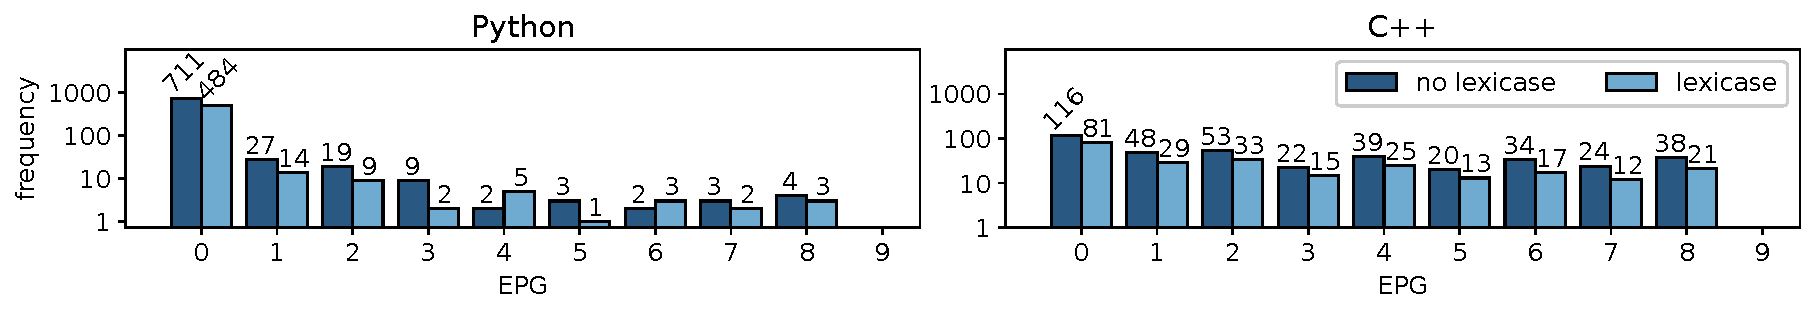
\includegraphics[width=\linewidth, trim={0mm 4mm 0mm 0mm}]{epg_distribution_humaneval_gpt35_1_01.pdf}
  \caption{HumanEval: 0 $\leq$ EPG $\leq$ 10 with step 1.}
  \label{fig:humaneval-epg-distrib-step-1}
\end{subfigure}
% 
\begin{subfigure}{\columnwidth}
\centering
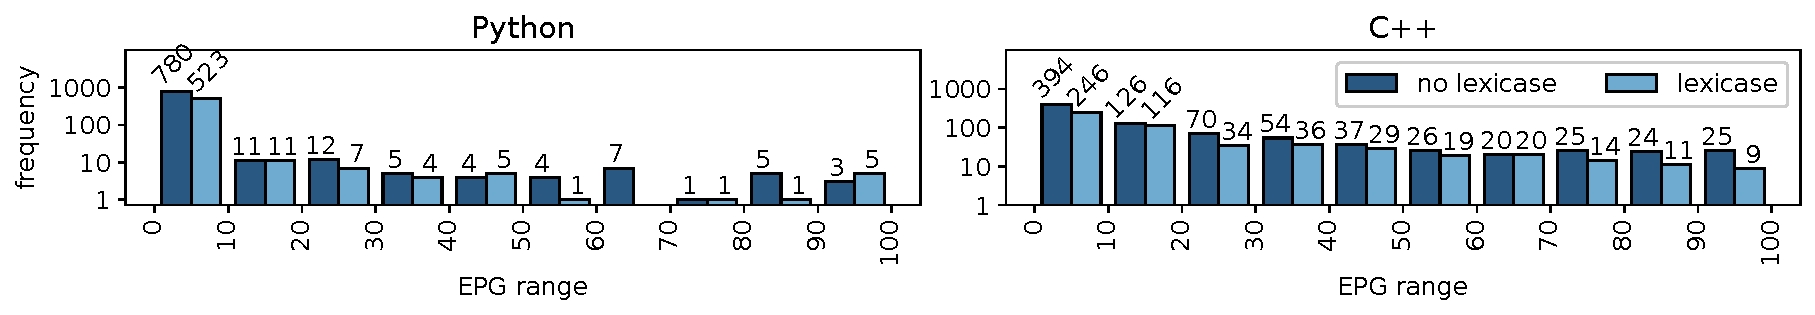
\includegraphics[width=\linewidth, trim={0mm 4mm 0mm 0mm}]{epg_distribution_humaneval_gpt35_10_01.pdf}
  \caption{HumanEval: 0 $\leq$ EPG $\leq$ 1000 with step 100.}
  \label{fig:humaneval-epg-distrib-step-10}
\end{subfigure}
\caption{Number of generated programs during each problem-solving attempt by tree arities $\treearitydraft{}, \; \treearitydebug{},$ }
\label{fig:epg-distribution}
\end{figure}

In the experiments where a solution was found, more runs without lexicase selection obtained $TPR=1$ earlier than the runs with lexicase selection (see figure~\ref{fig:epg-distribution}).
In general, out of 250 experiments for each language for PSB2, in 18.8\% of runs in Python and 33.2\% runs in C++, the draft program is already the solution (EPG=0). 
For 35.2\% of experiments in Python and 44.0\% runs in C++, the solution is found after discarding 5 candidates. 

The majority of experiments do not generate more than 10 programs. 
However, 8 PSB2 problems are solved with more than 50 generated programs in Python and in C++, 4 in each language.
By contrast, in HumanEval-X experiments, the problems are solved faster in Python than in C++, with 72.9\% tasks achieving $TPR=1$ with the draft solution in Python and 12.0\% tasks in C++.
Only 1.7\% experiments in Python reached a solution after discarding 50 candidates, while the analogical measure for C++ is 11.8\%.
Remarkably, although the speed of obtaining solution with $TPR=1$ in C++ is considerably lower, \method{} solved 12 more tasks in C++ (154) than in Python (142). 


% % TODO for extension: Are they the same tasks or different ones? Does seidr solves collectively more than other models or some uniqye problems than other models? 

The EPG distribution results for correctly solved problems with $TPR=1$ imply that the first steps in the update of the draft program are crucial for solving the problem. 
The chances of solving the problem on the later stages of the search are low.
This confirms our initial assumption in Section~\ref{sec:trade-off-settings} that 100 programs are sufficient.

Quality-diversity ranking strategy outperformed the average quality-first ranking in the Python experiments, both on PSB2 ($N^*=4, \;, 10, \; 16$) and HumanEval-Python ($N^*=2, \;, 10, \; 16$). 
To explore the impact of using quality-diversity over average quality-based ranking, we filter out the problems solved with more than one attempt and show the best average score described in Section~\ref{sec:execute} in figure~\ref{fig:avg-score-lexicase} for PSB2 and HumanEval-Python. 
We can see that the majority of problems are solved with a jump of average score from zero to one, except for one case in HumanEval-Python and two cases in PSB2 as shown by two angled lines in figure~\ref{fig:psb2-score-lexicase} and one such line in figure~\ref{fig:humaneval-score-lexicase}. 
These three experiments were the only cases where the ranking strategy worked. 
In other experiments with zero average scores reported up until the moment the solution is found, lexicase selection does not reorder the program candidates, which is also true for the majority of experiments with average quality-based ranking.

%%%%%%%%%%%%%%%%%%%%%%%%%%%%%%%%%%%%%%%%%%
% BEST AVG SCORE FOR LEXICASE IN  PYTHON
%%%%%%%%%%%%%%%%%%%%%%%%%%%%%%%%%%%%%%%%%%
\begin{figure}
 % trim={left lower right upper}
\begin{subfigure}{\textwidth}
\centering
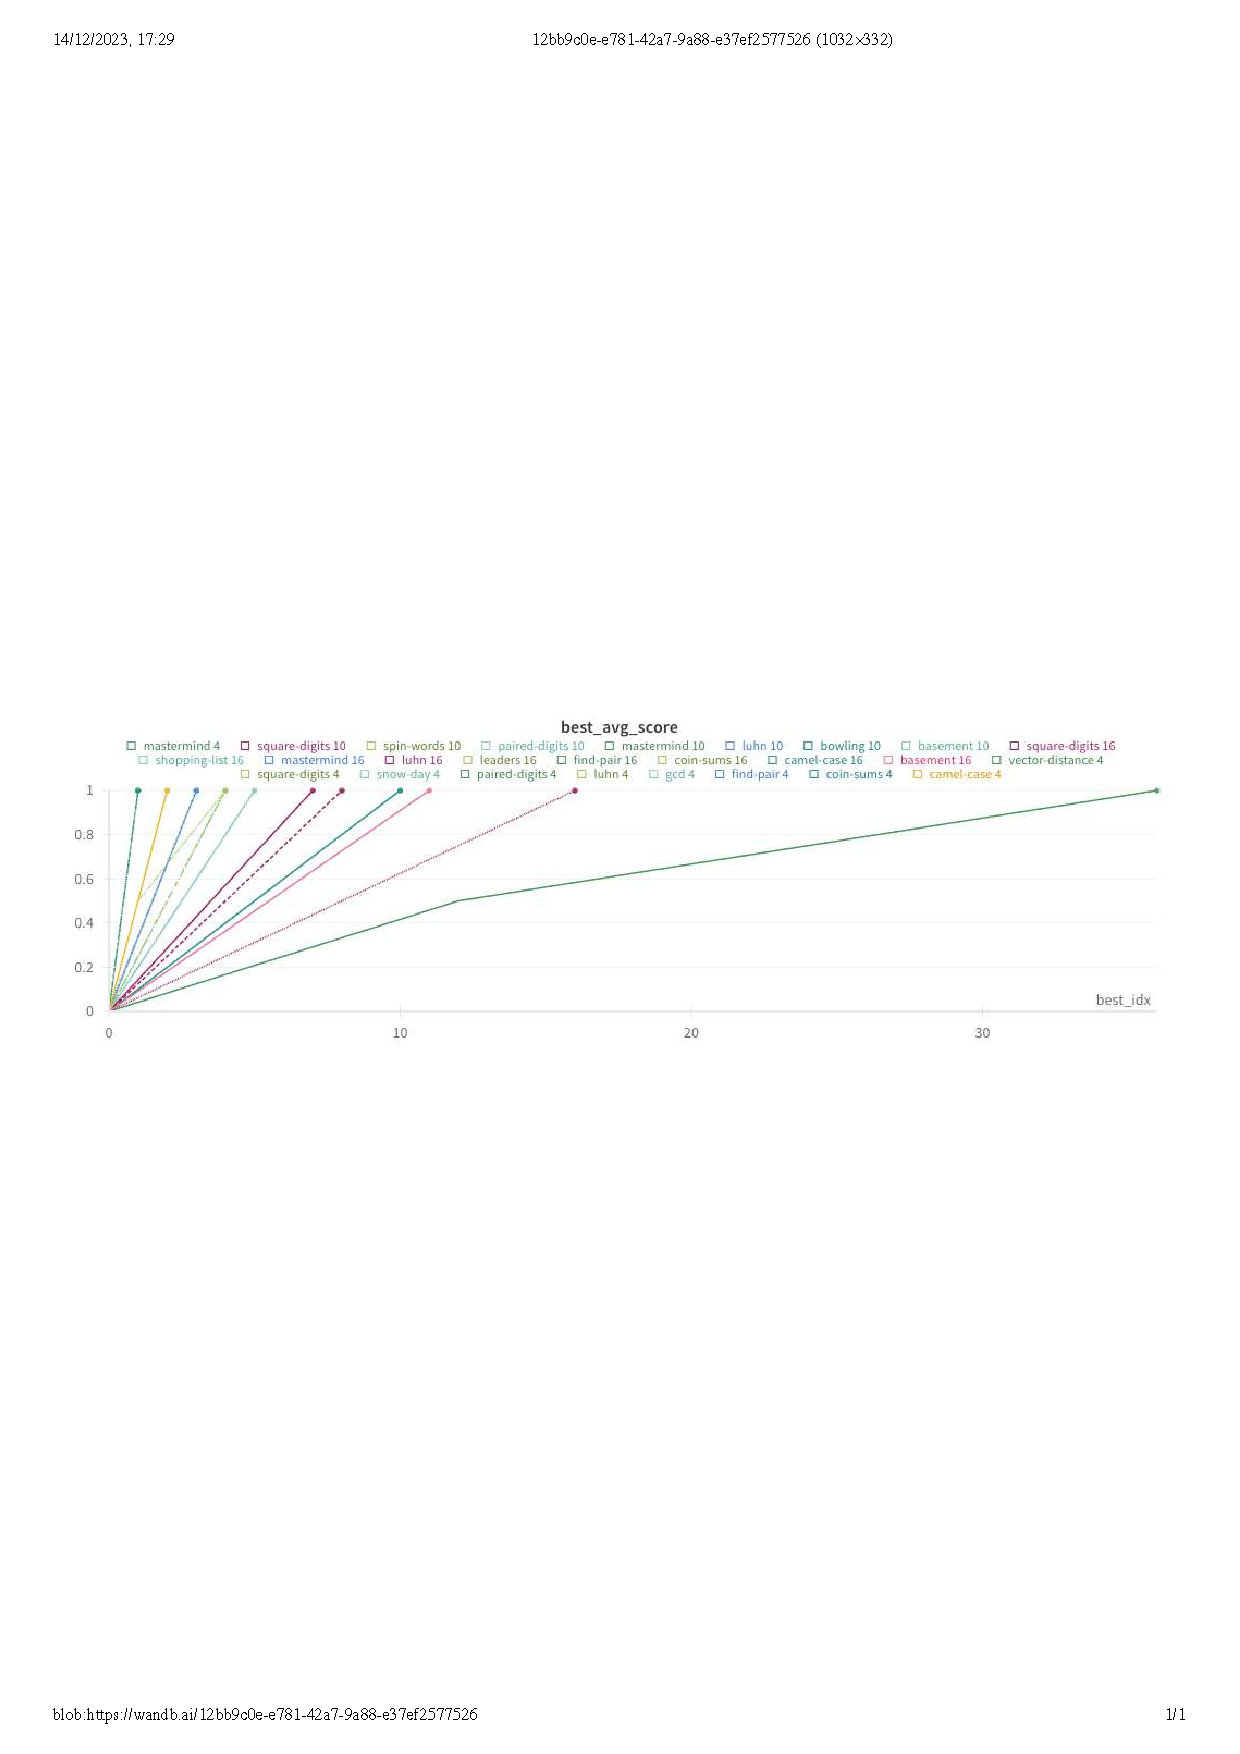
\includegraphics[width=.82\linewidth, trim={0mm 120mm 0mm 133mm}, clip]{lexicase-psb2-2_compressed.pdf}
  \caption{PSB2.}
  \label{fig:psb2-score-lexicase}
\end{subfigure}

% \vspace{2mm}

\begin{subfigure}{\textwidth}
\centering
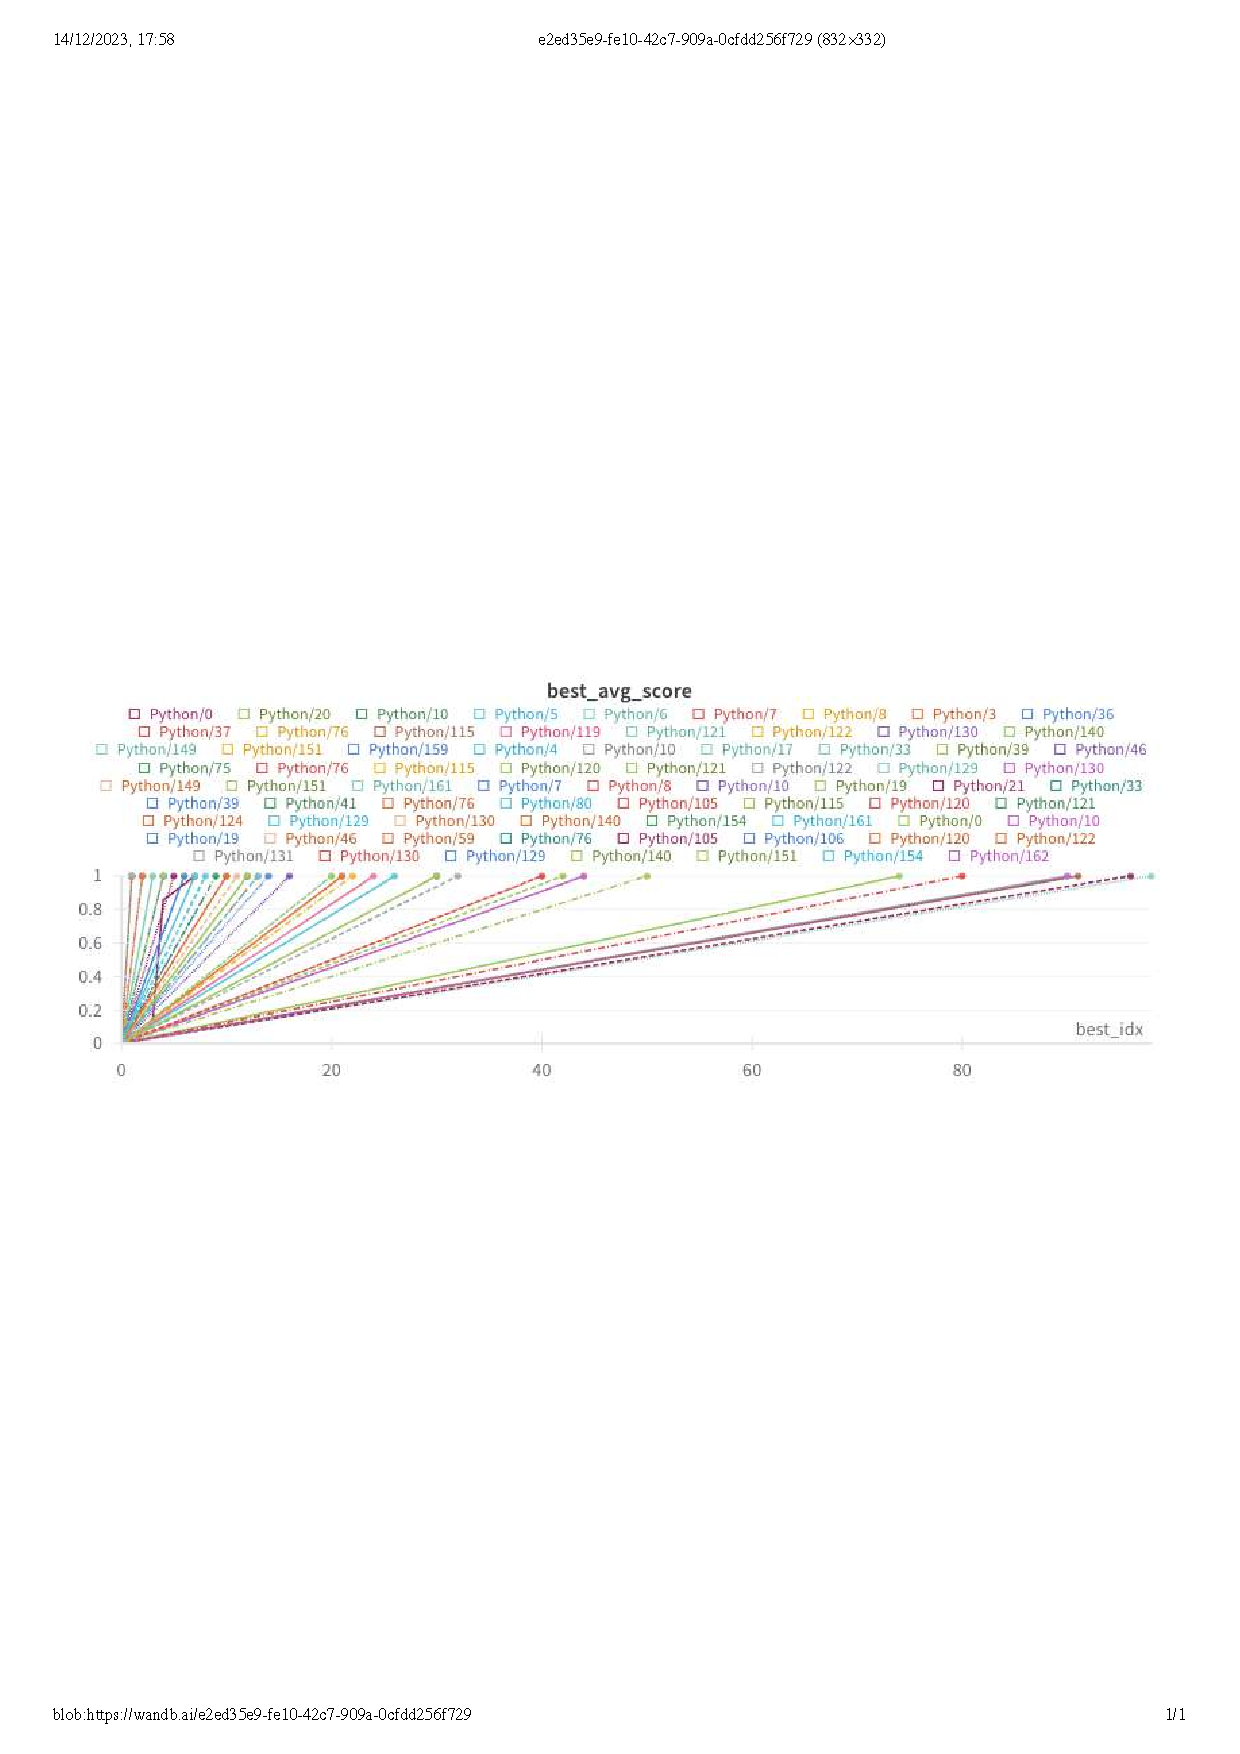
\includegraphics[width=.86\linewidth, trim={0mm 110mm 0mm 147mm}, clip]{lexicase-humaneval-2_compressed.pdf}
  \caption{HumanEval-Python.}
  \label{fig:humaneval-score-lexicase}
\end{subfigure}
% 
\caption{Rolling best average score for problems solved from the second or later attempts with lexicase selection.}
\label{fig:avg-score-lexicase}
% 
\end{figure}


% \begin{mdhighlight}[style=mystyle]
% \vspace*{-1mm}
% \noindent
\begin{highlight}
\textbf{Answer to RQ2: } 
While quality-diversity ranking outperforms average quality-first ranking in several Python experiments, the number of actual reranking steps performed is low. 
No leading ranking strategy is found for \method{} experiments with GPT-3.5 on PSB2 and HumanEval-X in Python and C++.
\end{highlight}
% \end{mdhighlight}
% \vspace*{-2mm}

\newpage \subsection{RQ3. Generalisability of \method{}}
\label{sec:results-rq3}

We choose the best performing tree arity for each benchmark and language to run \method{} with Code Llama 34B and compare the results to the findings for GPT-3.5 and Code Llama 34B without \method{} in table~\ref{tab:generalisability-psb2} for PSB2 and table~\ref{tab:generalisability-he} for HumanEval-X. 
The number of problems solved at different cutoffs ($k$) is reported for PSB2 and the percentage of solved problems at different $k$ is shown for HumanEval-X.
We compare the performance of PSB2 solutions synthesized with \method{} to the PushGP genetic programming system with down-sampled lexicase selection~\cite{helmuth2022:problemsolving}. 
For HumanEval-X, we cite the performance of the state-of-the-art models as reported by their authors without \method{}, such as CodeGeex~\cite{zheng2023:codegeex}, GPT-3.5 and GPT-4~\cite{openai2023:gpt4}, for reference, and compare \method{} with GPT-3.5 and CodeLlama results at different cutoffs ($k$ for $pass@k$).

In the PSB2 experiments, \method{} with GPT-3.5 and Code Llama 34B does not outperform \method{} with GPT-3, where Codex was used for code generation and repair steps. 
This finding suggests that using instruction models pre-trained for code generation is a better choice for  \synthesize{} and \debug{} agents of \method{}. 
\method{} with Code Llama performs worse than other models used in \method{} and does not solve any problem in Python. 
Closer inspection into generated candidate programs reveals that the model keeps generating near-misses which resemble correct code but do not pass tests.
Besides, during our experiments with Code Llama 34B loaded to ollama, we have found that the model needs frequent restarts. 

While \method{} with GPT-3.5 and Code Llama 34B does not outperform other state-of-the-art models, \method{} experiments with GPT-3.5 and $N^*<100,$ i.e., using repair steps as well as replacement as opposed to replacement-only evaluation, show consistently better results for GPT-3.5, which is also true for PSB2.  
Importantly, \method{}  with Code Llama 34B outperforms the current state-of-the-art model CodeGeeX, on HumanEval-C++ when comparing pass@10 achieving 77.44\% of solved tasks.
Moreover, \method{} with GPT-3.5 results in higher pass@100 than CodeGeeX: 93.29\% compared to 51.00\%. 

\begin{table}
    \centering
    \caption{Number of solved PSB2 problems using \method{} with different LLMs and PushGP. The best results among \method{}-only experiments at each $k$ are highlighted in bold. The best overall scores are underlined. If pass@100 is not available, the best reported results for a given method are mentioned in brackets.}\small
    \label{tab:generalisability-psb2}\vspace*{-4mm}
\begin{tabular}{llllrrr}
\toprule
Model & Language & $N^*$ & Ranking &  pass@1 &  pass@10 &  pass@100 \\
\midrule
 \method{} w/ GPT-3.5 & Python & 1   & average quality &       4 &        7 &         9 \\
&       & 2   & average quality &       6 &       11 &        12 \\
 &      &     & quality diversity  &       3 &        9 &         9 \\
 &      & 4   & average quality &       5 &        9 &        12 \\
&       &     & quality diversity  &       3 &       \textbf{12} &        13 \\
 &      & 10  & average quality &       6 &       10 &        12 \\
 &      &     & quality diversity  &       \textbf{7} &       \textbf{12} &        14 \\
 &      & 16  & average quality &       3 &       10 &        12 \\
 &      &     & quality diversity  &       6 &       \textbf{12} &        \textbf{15} \\
 &      & 100 & average quality &       4 &        5 &        14 \\
 \midrule
\method{} w/ Code Llama 34B & Python &  16  & quality diversity &    0 &        0 &         0 \\
 \method{} w/ GPT-3 & Python  & 10 & average quality &       - &        - &      (pass@1000=\underline{19}) \\
  \midrule
 PushGP & Python &  -   &    -            &       - &        - &      (\underline{17})\\
\midrule
\method{} GPT-3.5 & C++ & 1   & average quality &       9 &       12 &        12 \\
  &     & 2   & average quality &      \textbf{10} &       \textbf{14} &        14 \\
  &     &     & quality diversity  &       8 &       13 &        13 \\
  &     & 4   & average quality &       8 &       \textbf{14} &        \textbf{15} \\
  &     &     & quality diversity  &      \textbf{10} &       11 &        14 \\
  &     & 10  & average quality &       9 &       12 &        \textbf{15} \\
  &     &     & quality diversity  &       8 &       11 &        14 \\
  &     & 16  & average quality &      \textbf{10} &       13 &        \textbf{15} \\
  &     &     & quality diversity  &       7 &       11 &        14 \\
  &     & 100 & average quality &       4 &        4 &         8 \\
  \midrule
\method{} w/ Code Llama 34B & C++ &  16  & average quality  &    5 &        6 &         8 \\
\method{} w/ GPT-3 & C++  & 10 & average quality &       - &        - &      (pass@1000=\underline{17})\\
\midrule
PushGP & C++ &  -   &    -            &       - &        - &      (\underline{17})\\

\bottomrule
\end{tabular}
\end{table}




\begin{table}
    \centering
    \caption{Percentage of solved tasks for HumanEval-X using \method{} with different LLMs. The best results among \method{}-only experiments at each $k$ are highlighted in bold. The best overall scores are underlined. If pass@100 is not available, the best reported results are mentioned as in the corresponding chapters. }\small
    \label{tab:generalisability-he}\vspace*{-4mm}
\begin{tabular}{llllrrr}
\toprule
Model & Language & $N^*$ & Ranking &  pass@1 &  pass@10 &  pass@100 \\
\midrule
\method{} w/ GPT-3.5 & Python & 1   & average quality &   56.71 &    60.37 &     64.02 \\
&        & 2   & average quality &   \textbf{58.54 }&    63.41 &     67.07 \\
&        &     & quality diversity  &   54.27 &    56.71 &     59.15 \\
&        & 4   & average quality &   \textbf{58.54} &    \textbf{65.24} &     \textbf{68.90} \\
&        &     & quality diversity  &   54.88 &    59.76 &     61.59 \\
&        & 10  & average quality &   53.66 &    60.37 &     61.59 \\
&        &     & quality diversity  &   55.49 &    59.76 &     61.59 \\
&        & 16  & average quality &   \textbf{58.54} &    64.63 &     65.85 \\
&        &     & quality diversity  &   54.27 &    60.37 &     63.41 \\
&        & 100 & average quality &   56.10 &    57.32 &     64.02 \\
\midrule
\method{} w/ Code Llama 34 & Python & 4 &  average quality &   34.76 &    49.39 &     54.27 \\
\midrule
Code Llama 34B & Python & - &  - &  48.8  &  76.8   &    93.0 \\
Unnatural Code Llama 34B & Python & - &  - &  62.2  &  \underline{85.2}   &    \underline{95.4} \\
GPT-3.5 (ChatGPT) & Python & - &  - &  48.1  &  -   &    - \\
GPT-4 & Python & -&  - & \underline{67.0}   &  -   &    - \\
CodeGeeX & Python & - &  - &  22.89  &  39.57   &    60.92 \\
\midrule
 \method{} w/ GPT-3.5 & C++ & 1   & average quality &   10.98 &    67.68 &     \underline{\textbf{93.29}} \\
&        & 2   & average quality &   11.59 &    53.05 &     90.85 \\
&        &     & quality diversity  &   11.59 &    46.34 &     87.80 \\
&        & 4   & average quality &   \textbf{14.63} &    43.90 &     87.20 \\
&        &     & quality diversity  &   14.02 &    43.29 &     87.20 \\
&        & 10  & average quality &   12.80 &    31.10 &     73.17 \\
&        &     & quality diversity  &   12.20 &    31.71 &     70.12 \\
&        & 16  & average quality &    9.15 &    28.66 &     77.44 \\
&        &     & quality diversity  &   11.59 &    26.83 &     76.22 \\
&        & 100 & average quality &   10.98 &    14.63 &     64.63 \\
\midrule
\method{} w/ Code Llama 34B & C++ & 1 & average quality &    0.61 &    \underline{\textbf{77.44}} &     85.37 \\
\midrule
Code Llama 34 & C++ & - &  - &  \underline{47.8}  &  -   &    - \\
CodeGeeX & C++ & - &  - &  17.06  &  32.21   &    51.00 \\
\bottomrule
\end{tabular}
\end{table}

% \begin{mdhighlight}[style=mystyle]
% % \vspace*{-1mm}
% \noindent
\begin{highlight}
\textbf{Answer to RQ3:} 
The use of \method{} with GPT-3.5 outperforms the use of GPT-3.5 without \method{}, when the model is called with the same prompts as in \method{}: higher pass@k values are observed with $N^*<100$ than with $N^*=100.$ \method{} with Code Llama and GPT-3.5 does not outperform the current state-of-the-art results methods on PBS2, but does so for HumanEval-C++. 
\end{highlight}
% \end{mdhighlight}
% % \vspace*{-2mm}

\newpage \subsection{Threats to Validity}
\label{sec:threats}



External threats to validity concern \method{} performance on different other benchmarks and the use of more language models than the tested ones. 
Specifically, PSB2 and HumanEval-X contain programming tasks which require smaller functions to be generated than production-scale software.
While some canonical solutions provided in HumanEval-Python have been criticised~\cite{liuYourCodeGenerated2023}, we primarily use tests to evaluate the output of \method{}. Therefore, their weaknesses do not impact our results.
% We plan to extend our experiments in future work to explore the generalizability of results to more complex benchmarks.

Internal threats relate to the implementation.
We use PSB2, which has corner case tests in the training set and test regular cases in the test set. 
To ensure a fair comparison with other studies on PSB2, we evaluate and report results on the provided test set of PSB2 which risks that the synthesized programs do not pass some of the training cases. 
Large models for code editing and text completion used in this study are nondeterministic, which impacts results. 
Due to prohibitive model inference costs, each experiment was only run once.
However, our temperature sampling procedure described in section \ref{sec:synth} reduces this stochasticity significantly, especially for low-EPG results.
As with other language models, GPT-3.5 is a black-box model and may generate malicious code~\cite{pearceAsleepKeyboardAssessing2022}. 
The results can be skewed towards high performance in popular programming languages in the pre-training dataset used by authors of the tested LLMs.

\newpage \section{Conclusion}
\label{sec:conclusion}
In this study, we propose \method{}: a multi-agent framework to solve the challenge of fully autonomous programming. 
We augment the program synthesis procedure based on the large language models for code generation from templates and textual instructions with a \debug{} agent. 
The \debug{} agent performs tree search across the program candidates generated by a large language model for code.
The LLM used for code repair takes imperfect program candidates and instructions for their improvement as prompts. 
The instructions are obtained from both static templates with failing test case descriptions and templates with auto-generated bug summaries by a text completion language model. 
We explore 11 prompting strategies and the repair-replace trade-off of updating the draft program.

\head{Contributions}
We \method{} with GPT-3.5 and Code Llama 34B as the model for draft program synthesis, explaning errors in synthesized programs and their debugging in Python and C++ on the PSB2 and HumanEval-X benchmarks. 
In our experiments, \method{} does not outperform the state-of-the-art baselines for PSB2 and HumanEval-Python but shows better performance than using LLMs without \method{} with the same prompts as in \method{}.
\method{} achieves the state-of-the-art result for pass@10 (74.44\%) with Code Llama 34B and for pass@100 (93.29\%) with GPT-3.5 on HumanEval-C++. 
The approach requires under 100 program executions to obtain the reported results, 
% in stark contrast to billions\footnote{A problem is considered "solved" by PushGP if at least 1 of 100 runs, each with a limit of 60 million programs, was successful.} of executions in PushGP, 
making it feasible in the areas with costly testing, such as robotics.
Investigation of the repair-replace trade-off shows that \method{} with moderate number of generated programs for each bug explanation is favourable both for obtaining a solution and for the speed of solving a task. 
% Our prompt engineering study shows that bug summaries generated with ``confidence indicators'', such as ``obviously'', improve the performance of \method{} during C++ code synthesis. 
% Overall, our framework shows low performance variability with different prompts, which indicates its robustness.%

\head{Future work}
Further investigation of \method{} generalisability and ranking strategies are some of the areas for future work. 
Benchmarks with more tests than in HumanEval-X may shed more light on the most effective choice of the number of programs generated from each bug explanation, as well as the framework's comparison on large-context projects. 